% !TeX program = lualatex
\documentclass[]{article}
\usepackage{caption}
\usepackage{subcaption}
\usepackage{graphicx}
\usepackage{float}
\usepackage{url}
\usepackage{amsmath}
\usepackage{amssymb}
\usepackage{amsthm}
\usepackage{tocloft}
\usepackage{cancel}
\usepackage{thmtools}
\usepackage{gensymb}
\usepackage{braket}
\usepackage{tikz-feynman}
\usepackage{mathtools}
\usepackage{color}
\usepackage{colortbl}
\usepackage[toc,nonumberlist]{glossaries}
\usepackage{glossaries-extra}
\usepackage[toc,page]{appendix}

\newcommand\numberthis{\addtocounter{equation}{1}\tag{\theequation}}

\newtheorem{thm}{Theorem}
\newtheorem{defn}[thm]{Definition}
\newtheorem{cor}[thm]{Corollary}
\newtheorem{lemma}[thm]{Lemma}
\graphicspath{{figs/}}
\widowpenalty10000
\clubpenalty10000
\setcounter{tocdepth}{2}
\tikzfeynmanset{compat=1.1.0}
\definecolor{Gray}{gray}{0.5}
\DeclareMathOperator{\Tr}{Tr \;}
%opening
\title{Theoretical Minimum\\Quantum Entanglement, Part 1}
\author{Simon Crase (compiler)\\simon@greenweaves.nz}

\begin{document}

\maketitle

\begin{abstract}
These are my notes from the Quantum Entanglement Part 1, lectures\cite{susskind2013entanglement}  from Leonard Susskind's Theoretical Minimum series\cite{susskind2007theoretical}. Since the lectures were given weekly, Professor Susskind often repeats material from one lecture at the start of the next. I have omitted much of the repeated material.

	\begin{quotation}
		The old Copenhagen interpretation of quantum mechanics associated with Niels Bohr is giving way to a more profound interpretation based on the idea of quantum entanglement. Entanglement not only replaces the obsolete notion of the collapse of the wave function but it is also the basis for Bell's famous theorem, the new paradigm of quantum computing, and finally the widely discussed "many-worlds" interpretation of quantum mechanics originated by Everett--\cite{susskind2013entanglement}
	\end{quotation}

Disclaimer: I have created these notes as an aide-m\'emoire for my own use; if you find them useful, you are welcome, but I'd appreciate hearing from you. They are not intended as a substitute for listening to the lectures. The intellectual property for all material derived from the lectures belongs, of course, to Professor Susskind; any mistakes, however, are my own. I have added headings based on the topics covered in each lecture, since each of the original lectures has the same title, \emph{Quantum Entanglement}.

The notes were created using TeXstudio\cite{TexStudio}, and the bibliography with JabRef\cite{Jabref}.

\end{abstract}

\tableofcontents
\listoffigures
\listoftables
\listoftheorems[title=List of Theorems and Definitions]

\section{Introduction}

We, as animals, have inherited, through the process of evolution, certain intuitive ways of thinking about the physical world:
\begin{enumerate}
	\item a lioness, pursuing an antelope, will stop as soon as relative velocity changes sign (physics calculation!);
	\item a Neanderthal pushing a rock from the door of his cave aims body to maximize component of force in the right direction.
\end{enumerate}

Everything in modern physics has to do with those things that are beyond these intuitions: speeds approaching speed of light; 4 dimensions; the electron; the uncertainty principle. Why would natural selection have given us the intuition of the uncertainty principle? Intuitions for particles come from rocks.

This course will try to expose some of the weirdness of quantum mechanics, the weirdness of the logic of quantum mechanics, the weirdness of how quantum information works. 

This course will cover:
\begin{enumerate}
	\item the basic logic of quantum mechanics;
	\item the basic logic of quantum information theory;
	\item physics as information.
\end{enumerate}

Classical mechanics represents values as real numbers; QM often uses discrete values. Before we cover quantum bits we will look at classical bits, using Dirac's notation $\ket{0}$ or $\ket{1}$. For an n-bit \emph{classical} system, the number of configurations is $N_S=2^n$, so $n=\log_2(N_S)$.

We can generalize the definition of the number of bits of information: it doesn't have to be an integer. We can represent the state of a physical system, to a specified precision, by a string of bits (quantize space, etc). Figure \ref{fig:state_transition} shows how the laws of physics can be represented as a state transition diagram.

\begin{figure}[H]
	\caption[State transition diagram for laws of physics]{The laws of physics can be represented as a state transition diagram. In quantum mechanics there is no fundamental difference between forward in time and backward in time.}\label{fig:state_transition}
	\begin{subfigure}[t]{0.45\textwidth}
		\caption{A reversible law}\label{fig:state_transition_reversible}
		\begin{center}
			\begin{tikzpicture}[node distance=2cm]
			\node (A) at (0, 0) {};
			\node (B) at (0, 2) {};
			\node (C) at (2, 2) {};
			\node (D) at (2, 0) {};
			\draw[->]
			(A) edge (B) (B) edge (C) (C) edge (D) (D) edge (A);	
		\end{tikzpicture}
	\end{center}
	\end{subfigure}
	\begin{subfigure}[t]{0.45\textwidth}
		\caption{An irreversible law}
		\begin{center}
			\begin{tikzpicture}[node distance=2cm]
				
				% nodes
				\node (A) at (0, 0) {};
				\node (B) at (0, 2) {};
				\node (C) at (2, 2) {};
				\node (D) at (2, 0) {};
				
				% arrows
				\draw[->]
				(A) edge (B) (B) edge (C) (C) edge (D) ;
				\draw [->] (D)--(B); 
			\end{tikzpicture}
		\end{center}
	\end{subfigure}
\end{figure}

All real systems are quantum mechanical. In this course we will try to answer the question why the quantum mechanics is suppressed in many systems we observe.

\begin{defn}[A Newtonian system is one that is in a definite state, and that evolves deterministically]
\end{defn}

The Second Law of Thermodynamics arises because we lose the ability to follow the evolution of a system in precise detail.

LS reviews vectors and matrices:
\begin{itemize}
	\item Row and column vectors as sequences of number;
	\item Inner products;
	\item Matrices--linear transformation of vectors.
\end{itemize}

We can represent a state by a "one hot" vector, and then represent the transitions of, say, Figure \ref{fig:state_transition_reversible}, by a matrix of ones and zeros.

\section{Review of Quantum Mechanics}

This section reviews material from \cite{susskind2013quantum}.
\subsection{Spin of a single electron}

Classical mechanics is based on classical logic. Classical logic means that the states are Boolean: a set of points, each representing a state, and all the logic is classical. Quantum mechanics depends on a completely different logic.

We start with a quantum bit or Qbit, such as the spin of an electron. We need the concepts of \emph{preparing} a state, and \emph{detecting} a state.

\begin{itemize}
	\item Classically we can \emph{prepare} an electron to point in a particular direction by placing it in a magnetic field. The electron will precess before aligning: the stronger the field the faster it emits electromagnetic radiation and aligns.
	\item To \emph{detect} we apply magnetic field, and measure radiation to see how much realignment was needed.
\end{itemize}

This is \emph{not} the way a real electron works: no matter how we prepare a real electron, when we turn on the magnetic field, either:
\begin{itemize}
	\item nothing happens; or
	\item it emits a single photon corresponding to the flip from down to up.
\end{itemize}
It is almost as if the electron has only two possible configurations. But what if we prepare it at $45^\circ$ or $90^\circ$? Still we get up or down. What if we measure in some other direction?

What if we prepare up, turn off the field, and later measure? Up.

What if we prepare at $45^\circ$, turn off the field, then measure up/down? Then there is a probability of emitting photon. Probability has memory of previous state. Once you measure, state is fixed.

In physics we have learned not to ask questions unless we can devise a way to measure the answer.


\subsection{Spins of two Electrons}

\begin{itemize}
	\item The state space is an abstract vector space.

	\item LS reviews vector spaces, bras and kets, and represents the electron pointing up as $\ket{+}$. The general representation for an electron is $a_+\ket{+}+a_-\ket{-}$, where $a_+^*a_+$ is the probability that we will find the electron in the up state. Normalized vectors represent physical states.
	
	\item We have to rewire ourselves to understand QM.

	\item Linear combinations of states correspond to preparation in different directions.
	
	\item The two notions of vector (spatial and abstract) are related, but not simply.
	
	\item Anything that we can measure (with a number) is an observable.
	
	\item If we knew the rules for calculating averages for all possible observables, we would also know how to compute the probability distribution.
	
	\item Hermitian matrices are the quantum equivalent of observables.
	
\end{itemize}


\section{Postulates of Quantum mechanics}
\subsection{Review (continued)}
This section continues the review of material from \cite{susskind2013quantum}.

\begin{itemize}
	\item Complex numbers
	\item The equation $e^{i\theta} = \cos{\theta} + i \sin{\theta}$ contains all of trigonometry. As an example, LS showed that we can use it to retrieve the formula for $\cos(\theta+\phi)$.
\end{itemize}

\subsection{Postulates of Quantum mechanics}

\begin{enumerate}
	\item States are represented by normalized vectors.
	\item Observables are represented by Hermitian matrices.
	\item Expectation: $\bar{M}=\braket{a|M|a}$ - 
	\item Eigenvalues and Eigenvectors
\end{enumerate}


We need complex numbers to handle evolution with time.

\begin{defn}[Pauli Matrices]
	\begin{align*}
		\sigma_3 =& \begin{bmatrix} 1&0\\
			0&-1
		\end{bmatrix} \numberthis \label{eq:sigmas} \\
		\sigma_2 =& \begin{bmatrix}
			0 & -i\\
			i & 0
		\end{bmatrix}\\
		\sigma_1 =& \begin{bmatrix} 0&1\\
			1&0
		\end{bmatrix} \text{. We can show that}\\
		\sigma_3^2 =& 1 \numberthis \label{eq:sigma_sq}\\
		\sigma_2^2 =& 1\\
		\sigma_1^2 =& 1
	\end{align*}
\end{defn}

The eigenvalues are $\pm1$.


\begin{thm}[If $M$ is Hermitian,  the eigenvectors are real and orthogonal]
	\begin{align*}
		M =& M^\dagger \text{ and} \numberthis \label{eq:hermitian}\\
		M \ket{a} =& \lambda_a \ket{a} \numberthis \label{eq:sigma_ev1}\\
		\implies&\\
		\lambda_a =&\lambda_a^*
	\end{align*}
	In addition if
	\begin{align*}
		M \ket{b} =& \lambda_b \ket{b}\text{ and} \numberthis \label{eq:sigma_ev2}\\
		\lambda_a \ne& \lambda_b \text{ we have} \numberthis \label{eq:ne} \\
		\braket{a \vert b} =& 0 \numberthis \label{eq:orthogonal}
	\end{align*}
\end{thm}

\begin{proof}
	From (\ref{eq:sigma_ev1})
	\begin{align*}
		\braket{a \vert M \vert a} =& \lambda_a \braket{a\vert a} \text{, transposing}\\
		\braket{a \vert M^\dagger \vert a} =& \lambda_a^* \braket{a\vert a} \text{, then applying \eqref{eq:hermitian}} \\
		\braket{a \vert M \vert a} =& \lambda_a^* \braket{a\vert a} \text{, whence}\\
		\lambda_a^* =& \lambda_a
	\end{align*}
	Using  (\ref{eq:sigma_ev1}) again:
	\begin{align*}
		\braket{b \vert M \vert a} =& \lambda_a \braket{b\vert a} \text{, and from (\ref{eq:sigma_ev2})}\\
		\braket{a \vert M \vert b} =& \lambda_b \braket{a\vert b} \text{, or, using (\ref{eq:hermitian})}\\
		\braket{b \vert M \vert a} =& \lambda_b \braket{b\vert a} \text{, whence}\\
		(\lambda_1-\lambda_b)\braket{b\vert a} =& 0 \text{, so, using (\ref{eq:ne})}\\
		\braket{b\vert a} =& 0\text{, which is (\ref{eq:orthogonal})}
	\end{align*}
\end{proof}

\section{Spins \& Quantum Entanglement}

\subsection{Review of spins of single electrons (continued)}

Consider spin about an arbitrary "pointer" $(n_1,n_2,n_3)$

\begin{align*}
	\vec{\hat{n}}\cdot\vec{\sigma} =& n_1\sigma_1 + n_2\sigma_2 + n_3 \sigma_3\\
	=& \begin{bmatrix}
		n_3&n_1-i n_2\\
		n_1 + i n_2&-n_3
	\end{bmatrix} \text{, where $n_1^2 + n_2^2 +n_3^2 = 1$}
\end{align*}
We define:
\begin{align*}
	n_1-i n_2 =& n_-\\
	n_1+i n_2 =& n_+\text{ then}\\
	\vec{\hat{n}}\cdot\vec{\sigma} =&\begin{bmatrix}
		n_3&n_-\\
		n_+&-n_3 
	\end{bmatrix}
\end{align*}
$\vec{\hat{n}}\cdot\vec{\sigma}$ is Hermitian, hence an observable (turn on magnetic field along $\vec{n}$). We can show that $(\vec{\hat{n}}\cdot\vec{\sigma})^2=I$, whence its eigenvalues are $\pm 1$. Moreover
\begin{align*}
	n_+ n_- =& n_1^2 + n_2^2 + n_3^2 -n_3^2\\
	=& 1 - n_3^2 \numberthis \label{eq:n3:2}
\end{align*}

Figure \ref{fig:et-4-1} depicts the only interesting question we can ask about a single spin:  if we prepare along one axis, measure along another, what is the probability of positive versus negative?

\begin{figure}[H]
	\caption{Prepare Spin along $\vec{\hat{n}}$, measure along $\vec{\hat{m}}$}\label{fig:et-4-1}
	\begin{center}
		\begin{tikzpicture}[node distance=2cm]
			\node (A) at (0, 0) {};
			\node (B) at (0.2, 2) {};
			\node (C) at (1.414, 1.414) {};
			\draw [->] (A)--(B) node[above] {$\vec{\hat{m}}$}; 
			\draw [->] (A)--(C) node[above] {$\vec{\hat{n}}$};
		\end{tikzpicture}
	\end{center}
\end{figure}

We need the eigenvectors of $\vec{\sigma} \cdot \vec{\hat{n}}$ and   $\vec{\sigma} \cdot \vec{\hat{m}}$.
We have:
\begin{align*}
	(\vec{\sigma} \cdot \vec{\hat{n}}) \ket{\vec{\sigma} \cdot \vec{\hat{n}}=1} =& 1 \ket{\vec{\sigma} \cdot \vec{\hat{n}}=1} \text{ and}\\
	(\vec{\sigma} \cdot \vec{\hat{m}}) \ket{\vec{\sigma} \cdot \vec{\hat{m}}=1} =& 1 \ket{\vec{\sigma} \cdot \vec{\hat{m}}=1}
\end{align*}

We need the probability amplitude that, if you prepare with $\vec{\sigma} \cdot \vec{\hat{n}}=1$ and then measure along $\vec{\hat{m}}=$ we will observe $\vec{\sigma} \cdot \vec{\hat{m}}=1$:
$$P(\vec{\sigma} \cdot \vec{\hat{m}}=1\vert\vec{\sigma} \cdot \vec{\hat{n}}=1) = \vert \braket{\vec{\sigma} \cdot \vec{\hat{m}}=1\vert\vec{\sigma} \cdot \vec{\hat{n}}=1}\vert^2$$.

This is what quantum mechanics does: it answers the question, "What is the probability I'll get a measurement of this value, given that I prepared the experiment is such and such a manner?"

To calculate the eigenvectors of $\vec{\sigma} \cdot \vec{\hat{n}}$, we start:
\begin{align*}
	\begin{bmatrix}
		n_3 &n_-\\
		n_+&-n_3
	\end{bmatrix}\begin{bmatrix}
		\alpha\\
		\beta
	\end{bmatrix}=&\begin{bmatrix}
		\alpha\\
		\beta
	\end{bmatrix}
\end{align*}
At this state we won't bother about normalization. (NB. Any vector can be multiplied by a phase: This has no physical effect: since $e^{i\theta}e^{-i\theta}=1$, the phase has no effect on any probabilities we calculate). We will arbitrary set: 
\begin{align*}
	\alpha=&1\\
	\beta=&z \text{, then our equation becomes}\\
	\begin{bmatrix}
		n_3 &n_-\\
		n_+&-n_3
	\end{bmatrix}\begin{bmatrix}
		1\\
		z
	\end{bmatrix}=&\begin{bmatrix}
		1\\
		z
	\end{bmatrix} \text{, whence}\\
	n_3 + n_- z =& 1 \text{, second line of multiplication gives the same result, so we'll ignore.}\\
	z =& \frac{1-n_3}{n_-} \text{, so our eigenvector becomes:}\\
	&\begin{bmatrix}
		1\\
		\frac{1-n_3}{n_-} 
	\end{bmatrix}
\end{align*}
The norm of the eigenvector is:
 \begin{align*}
 	1+\frac{1-n_3}{n_+}\frac{1-n_3}{n_-}=& \frac{n_+n_- + (1-n_3)^2 }{n_+n_-}\\ 
 	=&\frac{n_+n_- + 1 -2 n_3 + n_3^2}{n_+n_-} \text{. Now we use \eqref{eq:n3:2}}\\
 	=& \frac{1-\cancel{n_3^2}+1 - 2n_3 +\cancel{n_3^2}}{1-n_3^2}\\
 	=& \frac{2\cancel{(1-n_3)}}{\cancel{(1-n_3)}(1+n_3)} \text{, whence the normalized eigenvector is:}\\
 	\ket{\vec{\sigma} \cdot \vec{\hat{n}}=1} =& \sqrt{\frac{1+n_3}{2}} \begin{bmatrix}
 		1\\\frac{1-n_3}{n_-}
 	\end{bmatrix} \numberthis \label{eq:eigenvector:normalized}
 \end{align*}

Eventually we find:
\begin{align*}
	\vert \braket{\vec{\sigma} \cdot \vec{\hat{m}}=1\vert\vec{\sigma} \cdot \vec{\hat{n}}=1}\vert =& \frac{1 + \vec{\hat{n}} \cdot \vec{\hat{m}}}{2}\\
	=& \frac{1 + \cos{\theta_{mn}}}{2}
\end{align*}
We would get the same result if we rotated the experiment.

We can orient the system along any axis, and measure along any axis. We don't get fractional answers, we get fractional probabilities.

When you measure something, you go into system, interact with it, and \emph{change its state.} You leave the system in the eigenstate that corresponds to the measurement. Can we perform an experiment that measures spin along $\sigma_1$ and $\sigma_2$ simultaneously? No, because $\sigma_1$ and $\sigma_2$ don't share eigenvalues. For simultaneous measurement to be possible, need to share eigenvectors, i.e. if they \emph{commute}.

\begin{thm}[For simultaneous measurement to be possible, operators must commute.]
	\begin{align*}
			A\ket{\alpha_i} =& \lambda_i \ket{\alpha_i} \text{ and} \numberthis \label{eq:simultaneous1}\\
			B\ket{\alpha_i} =& \mu_i \ket{\alpha_i} \numberthis\label{eq:simultaneous2}\\
			\iff &\\
			AB - BA =& 0& \numberthis \label{eq:simultaneous3}\\
			[A,B] =& 0
	\end{align*}
\end{thm}

\begin{proof}
	From (\ref{eq:simultaneous1})
	\begin{align*}
		B A\ket{\alpha_i} =& \lambda_i B \ket{\alpha_i}\\
		=& \lambda_i \mu_i \ket{\alpha_i} \text{, from (\ref{eq:simultaneous2})} \text{. Similarly}\\
		A  B \ket{\alpha_i} =& \mu_i  \lambda_i \ket{\alpha_i} \text{, whence}\\
		B A\ket{\alpha_i} =& A  B \ket{\alpha_i} \text{ for every eigenvector $\ket{\alpha_i}$}
	\end{align*}
\end{proof}
\begin{thm}[Any direction corresponds to an axis of spin]\label{thm:any:direction:corresponds}
	For any $\alpha$ and $\beta$ such that $\alpha^2$ + $\beta^2=1$, there exists a direction of space such that $(\alpha, \beta)$ is an eigenvector of $\vec{\sigma} \cdot\vec{\hat{n}}$ with eigenvalue 1.
\end{thm}
\begin{proof}
	See \ref{proof:any:direction:corresponds}
\end{proof}
\subsection{Pairs of electrons--Entanglement at last}
There are four states: $\ket{u\;u}, \,\ket{d\;u}, \,\ket{u\;d}, \,\ket{d\;d}$.  We will use $\sigma$ for the first electron, $\tau$ for the second:  $\sigma$ leaves the second spin unchanged, $\tau$ leaves the first unchanged.

How many ways to combine? 
\begin{itemize}
	\item There are 4 complex parameters, so 8 real ones;
	\item But we can multiply any vector by a complex phases without affecting probabilities. so this adds a constraint to the real parameters;
	\item We need to normalize, which adds a second constraint.
	\item So the number of combinations is 8-2 = 6, but this is more than we'd expect from $2\times2$!
	\item The state space is richer than we'd expect. 
	\item This is entanglement!
\end{itemize}


The following \emph{product state} corresponds to a situation where the first electron has been carefully placed in one state, and the second in another.
\begin{align*}
	\big[\alpha_1\ket{u} + \beta_1\ket{d}\big]\big[\alpha_2\ket{u} + \beta_2\ket{d}\big] =& \alpha_1 \alpha_2 \ket{uu} + \alpha_1 \beta_2 \ket{ud} + \beta_1 \alpha_2 \ket{du} + \beta_1 \beta_2 \ket{dd}
\end{align*}
In such a case, there is always one direction in which the spin of the first electron is up, and similarly for the second electron (generally a different direction). LS exhibited an example where this is not true.

\begin{align*}
	\frac{1}{\sqrt{2}}\big[\ket{ud}+\ket{du}\big] \numberthis \label{eq:T1}
\end{align*}

If one electron is up, the other is down, and vice versa. We can learn something about one electron by measuring the other!.

\begin{thm}[Any $\sigma_i$ or $\tau_i$ acts on the expression (\ref{eq:T1}) to give zero]
	\begin{align*}
		\big[\bra{ud}+\bra{du}\big]\sigma_i\big[\ket{ud}+\ket{du}\big]=&0 \text{ and}\\
		\big[\bra{ud}+\bra{du}\big]\tau_i\big[\ket{ud}+\ket{du}\big]=&0
	\end{align*}
\end{thm}
\begin{proof}
	We shall prove for $\sigma_i$ only: the proof for $\tau_i$ is analogous.
	\begin{align*}
		\big[\bra{ud}+\bra{du}\big]\sigma_1\big[\ket{ud}+\ket{du}\big]=&\big[\bra{ud}+\bra{du}\big]\big[\ket{dd}+\ket{uu}\big]\\
		=&\braket{ud\vert dd} + \braket{ud\vert uu} + \braket{du\vert dd} + \braket{du\vert uu}\\
		=&0 \text{, since each term is zero.}
	\end{align*}
	Similarly:
	\begin{align*}
		\big[\bra{ud}+\bra{du}\big]\sigma_2\big[\ket{ud}+\ket{du}\big]=&i\big[\bra{ud}+\bra{du}\big]\big[\ket{dd}-\ket{uu}\big]\\
		=&i\braket{ud\vert dd} - \braket{ud\vert uu} + \braket{du\vert dd} - \braket{du\vert uu}\\
		=&0
	\end{align*}
	Finally:
	\begin{align*}
		\big[\bra{ud}+\bra{du}\big]\sigma_3\big[\ket{ud}+\ket{du}\big]=&\big[\bra{ud}+\bra{du}\big]\big[\ket{ud}-\ket{du}\big]\\
		=& \braket{ud\vert ud} - \braket{ud\vert du} + \braket{du\vert ud} - \braket{du\vert du}\\
		=& 1 -0 -0 -1\\
		=&0
	\end{align*}
\end{proof}
\begin{cor}[The probability of a spin being $+1$ (or $-1$) along any axis is $\frac{1}{2}$]
	$\vec{\sigma}\cdot\vec{\hat{n}}$ and $\vec{\tau}\cdot\vec{\hat{n}}$ both  act on the expression (\ref{eq:T1}) to give zero; hence the probability of a spin being $+1$ (or $-1$) along any axis is $\frac{1}{2}$.
\end{cor}

This is very different from two independent electrons.

\section{Bell's Theorem}

\subsection{Einstein-Podolsky-Rosen Correlation}

If we have two spins there are two interesting cases:
\begin{align*}
	\frac{1}{\sqrt{2}}\big[\ket{ud}\pm\ket{du}\big] \numberthis \label{eq:T1a}
\end{align*}
There is no way that either electron has a definite polarization. To see the difference between plus and minus in (\ref{eq:T1a}), consider the operator $\vec{\sigma} + \vec{\tau}$

\begin{align*}
	\big(\vec{\sigma_z} + \vec{\tau_z}\big)\frac{1}{\sqrt{2}}\big[\ket{ud}\pm\ket{du}\big]=& 0\\
	\big(\vec{\sigma_x} + \vec{\tau_x}\big)\frac{1}{\sqrt{2}}\big[\ket{ud}+\ket{du}\big]=& 2 \big[\ket{uu}+\ket{dd}\big]\\
	\big(\vec{\sigma_x} + \vec{\tau_x}\big)\frac{1}{\sqrt{2}}\big[\ket{ud}-\ket{du}\big]=& 0\\
	\big(\vec{\sigma_y} + \vec{\tau_y}\big)\frac{1}{\sqrt{2}}\big[\ket{ud}-\ket{du}\big]=& 0
\end{align*}
So, for the singlet state, $\frac{1}{\sqrt{2}}\big[\ket{ud}\pm\ket{du}\big]$, if we measure $\vec{\sigma}$ we know $\vec{\tau}$. (Einstein, Podolsky, Rosen)\cite{einstein1935can}

\subsection{Bell's Theorem and Bell's Inequality}\label{sec:bell}

We now come to Bell's famous theorem\cite{bell1964einstein}. Is it profound or trivial? Sometimes it seems profound, at other times it just seems to be a consequence of quantum mechanics. John Bell and Richard Feynman shared this ambivalence. The theorem is absolutely classical:  Bell's theorem excludes quantum mechanics; in quantum mechanics you can find violations of Bell's inequality.

NB: entanglement doesn't violate causality; we can't use it to send an instantaneous message from Alice to Bob. Bob has to receive a message from Alice in order to use his measurement.

\begin{thm}[Bell's Theorem]
We consider the class of objects that have certain properties $A$, $B$, and $C$.
	\begin{align*}
		N(A, \neg B) + N(B, \neg C) \ge N(A,\neg C)\text{,  Bell's inequality} \numberthis \label{eq:bell:inequality}
	\end{align*}
\end{thm}

Figure \ref{fig:bell} illustrates the theorem.
\begin{figure}[H]
	\caption{Venn Diagram for Bell's Inequality--\cite{wiki2020bell}}\label{fig:bell}
	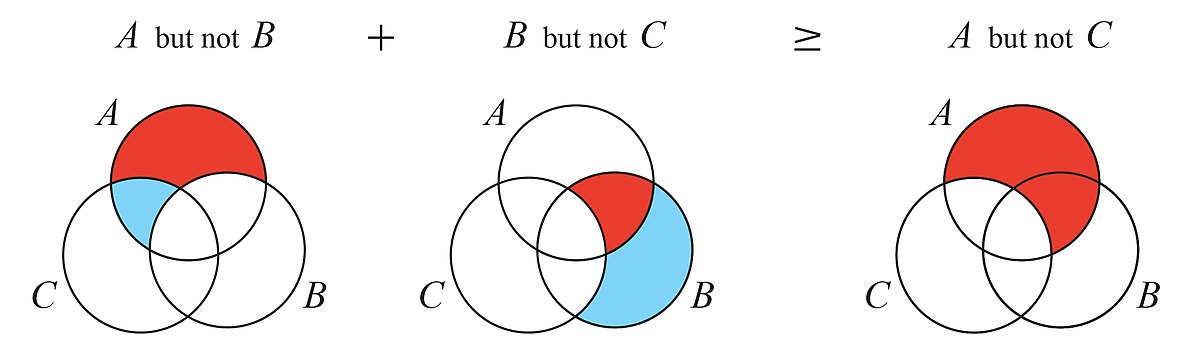
\includegraphics[width=0.8\textwidth]{1200px-Bell's_Theorem_JCB.jpg}
\end{figure}

\begin{proof}

    Table \ref{table:possibilities} depicts 8 possibilities for an object, which either has or does not have properties $A$, $B$, and $C$.
  
	\begin{table}[H]
		\caption[Bell's Theorem]{Bell's Theorem: each object either has or does not have properties $\{A, B,  C\}$. Each combination of properties is assigned a value chosen from the numbers 1 through 8. This table shows whether or not each combination contributes to the three sets $A \cap \neg B$, $B \cap \neg C$, and $A \cap \neg C $.}\label{table:possibilities}
		\begin{center}
			\begin{tabular}{|c|c|c|c|c|c|c|} \hline
				\#&$A$&$B$&$C$&$A \cap \neg B$&$B \cap \neg C$& $A \cap \neg C $\\ \hline
				\rowcolor{Gray}
				1&+&+&+&-&-&-  \\ \hline 
				2&+&+&-&-&+&+  \\ \hline
				3&+&-&+&+&-&-  \\ \hline 
				4&+&-&-&+&-&+  \\ \hline
				\rowcolor{Gray}
				5&-&+&+&-&-&-  \\ \hline 
				6&-&+&-&-&+&-  \\ \hline
				\rowcolor{Gray}
				7&-&-&+&-&-&-  \\ \hline
				\rowcolor{Gray} 
				8&-&-&-&-&-&- \\ \hline
			\end{tabular}
		\end{center}
	\end{table}

	From Table \ref{table:possibilities} we read off:
	\begin{align*}
		A \cap \neg B =& \{3, 4\} \\
		B \cap \neg C =& \{2, 6\} \text{, whence}\\
		(A \cap \neg B) \cup (B \cap \neg C) =&\{2,3,4, 6\}\\
		A \cap \neg C =& \{2,4\} \text{, from Table \ref{table:possibilities} }\\
		\subset& \{2,3,4, 6\} \text{, whence}\\
		A \cap \neg C \subset&(A \cap \neg B) \cup (B \cap \neg C)
	\end{align*}
Equation (\ref{eq:bell:inequality}) follows on taking the cardinalities of all three sets.
\end{proof}
What is amazing is that Bell's Inequality can be violated! One of the students said that the \emph{violation} is profound: but \emph{all} of QM violates classical mechanics. 

We now take our system to be two spins, and we will define $A$, $B$, and $C$. We will start by assuming classical spins, and that they can be measured as classical objects, and we will write down Bell's inequality. We will talk only about spin 1. A proposition might be: spin 1 is up along the z axis. The negative would be "spin 1 is not up along the z-axis, i.e. down", which is equivalent to "spin 2 is up" (in the Singlet state).

If classical logic made any sense we would measure (we have a beam of electron pairs. zillions of pairs, each of which are correlated) the first 100,000 in every possible manner, and we convince ourselves that the spins in each pair are opposite to each other. So the negative of "A is up" is "B is up."

\begin{table}[H]
	\caption{States for Classical Bell's inequality}\label{table:classical:bell}
	\begin{center}
		\begin{tabular}{|l|l|l|}\hline
			\#&Propositions& Negated\\ \hline 
			A&1 $\ket{u}$ along z axis&2 $\ket{u}$ along z axis\\ \hline
			B&1$ \ket{u}$ along $45^{\circ}$ angle in zx plane&2 $\ket{u}$ along $45^{\circ}$ angle in zx plane\\ \hline
			C&1 $\ket{u}$ along $90^{\circ}$ angle in zx plane&2  $\ket{u}$ along $90^{\circ}$ angle in zx plane\\ \hline
		\end{tabular}
	\end{center}
\end{table}

If the entities are pairs of electrons,  and we use the rotational invariance of the Singlet, the left hand side of (\ref{eq:bell:inequality}) becomes:
\begin{align*}
	\underbrace{N(A, \neg B)}_\text{1 up along z, 2 up along $45^\circ$} + \underbrace{N(B, \neg C)}_\text{N(A, \neg B) rotated $45^{\circ}$} =& 2N(A, \neg B)
\end{align*}
The right hand side is 1 up along z, 2 up along $90^\circ$, so we have something we can test.
\begin{align*}
	2N(\text{1 up along z, 2 up along $45^\circ$}) \ge N(\text{1 up along z, 2 up along $90^\circ$}) \numberthis \label{eq:bell:ineq:classical}
\end{align*}
Note that we can replace numbers with probabilities, since we are working with zillions of electrons. When we calculate the probabilities for the singlet state, we find that the $\ge$ sign in (\ref{eq:bell:ineq:classical}) comes out <, violating Bell's inequality. To calculate efficiently, we require projection operators.

\begin{align*}
	\mathbb{P}_{\sigma_i} =& \frac{\sigma_i + I}{2} \text{, for $i \in \{1,2, 3\}$}
\end{align*}

\begin{defn}[Alternative definition  for probability postulate of quantum mechanics]
	If we have an arbitrary state $\psi$, and we want the probability that a certain thing is true, construct the projection operator for the eigenvector corresponding to that certain thing, $\mathbb{P}$; the probability is the expectation of $\mathbb{P}$, $\braket{\psi|\mathbb{P}|\psi}$.
\end{defn}

\begin{enumerate}
	\item Projection operators correspond to statements.
	\item In classical physics, properties are subsets: the set of all things \emph{such that}...; we use classical logic.
	\item In quantum mechanics properties correspond to subspaces of a vector space; they are different from subsets of a set. 
\end{enumerate}

We'll recast Table \ref{table:classical:bell} in terms of projection operators.
\begin{table}[H]
	\caption{Projection operators for Bell's inequality}\label{table:projection:bell}
	\begin{center}
		\begin{tabular}{|l|l|l|l|}\hline
			\#&Proposition&Projection & Projection Negated\\ \hline 
			A& $\ket{u}$ along z axis&$\frac{1}{2}\big(\sigma_3 + I\big)$&\\ \hline
			B&$ \ket{u}$ along $45^{\circ}$ angle in zx plane&$\frac{1}{2}\big(\frac{\sigma_1+\sigma_3}{\sqrt{2}}+I\big)$&$\frac{1}{2}\big(\frac{\tau_1+\tau_3}{\sqrt{2}}+I\big)$\\ \hline
			C&$ \ket{u}$ along $90^{\circ}$ angle in zx plane&&$\frac{1}{2}\big(\tau_1+1\big)$\\ \hline
		\end{tabular}
	\end{center}
\end{table}

\subsubsection{Example calculation for violation of Bell's Inequality}

From Table \ref{table:projection:bell}, $P(A, \neg B) = \frac{1}{4}\big(\sigma_3 + I\big) \big(\frac{\tau_1+\tau_3}{\sqrt{2}}+I\big)$. Applying this to the Singlet, and using rotational invariance, the left side of (\ref{eq:bell:ineq:classical}) becomes:

\begin{align*}
	2& \frac{1}{\sqrt{2}}\big[\bra{ud}-\bra{du}\big]\frac{1}{4}\big(\sigma_3 + I\big) \big(\frac{\tau_1+\tau_3}{\sqrt{2}}+I\big)\frac{1}{\sqrt{2}}\big[\ket{ud}-\ket{du}\big]\\
	=& 2 \frac{1}{\sqrt{2}} \frac{1}{4} \frac{1}{\sqrt{2}} \big[\bra{ud}-\bra{du}\big]\big(\sigma_3 + I\big) \big(\frac{\tau_1+\tau_3}{\sqrt{2}}+I\big)\big[\ket{ud}-\ket{du}\big]\\
	=&\frac{1}{4} \big[\bra{ud}-\bra{du}\big]\big(\sigma_3 + I\big) \big(\frac{\tau_1+\tau_3}{\sqrt{2}}+I\big)\big[\ket{ud}-\ket{du}\big] \numberthis \label{eq:bell:lhs}
\end{align*}
We will build this expression up:
\begin{align*}
	\tau_3 \ket{ud} =& -\ket{ud}\\
	\tau_1 \ket{ud} =& \ket{uu}\\
	\tau_3 \ket{du} =& \ket{du}\\
	\tau_1 \ket{du} =& \ket{dd} \text{, whence}\\
	\big(\frac{\tau_1+\tau_3}{\sqrt{2}}+I\big)\ket{ud}=&\frac{\ket{uu}-\ket{ud}}{\sqrt{2}}+\ket{ud}\\
	=& \frac{\ket{uu}}{\sqrt{2}} + \big(1-\frac{1}{\sqrt{2}}\big)\ket{ud} \text{, and}\\
	\big(\frac{\tau_1+\tau_3}{\sqrt{2}}+I\big)\ket{du}=&\frac{\ket{dd}+\ket{du}}{\sqrt{2}}+\ket{du}\\
	=&\frac{\ket{dd}}{\sqrt{2}} + \big(1+\frac{1}{\sqrt{2}}\big)\ket{du}
\end{align*}
We now apply $\sigma_3 + I$:
\begin{align*}
	\big(\sigma_3 + I\big) \big(\frac{\tau_1+\tau_3}{\sqrt{2}}+I\big)\ket{ud}=&\big(\sigma_3 + I\big) \big[\frac{\ket{uu}}{\sqrt{2}} + \big(1-\frac{1}{\sqrt{2}}\big)\ket{ud}\big]\\
	=& 2 \big[\frac{\ket{uu}}{\sqrt{2}} + \big(1-\frac{1}{\sqrt{2}}\big)\ket{ud}\big] \text{, and}\\
	\big(\sigma_3 + I\big) \big(\frac{\tau_1+\tau_3}{\sqrt{2}}+I\big)\ket{du}=&\big(\sigma_3 + I\big) \big[\frac{\ket{dd}}{\sqrt{2}} + \big(1+\frac{1}{\sqrt{2}}\big)\ket{du}\big]\\
	=& 0
\end{align*}
So (\ref{eq:bell:lhs}) becomes:
\begin{align*}
	\frac{1}{4} \big[\bra{ud}-\bra{du}\big]  2 \big[\frac{\ket{uu}}{\sqrt{2}} + \big(1-\frac{1}{\sqrt{2}}\big)\ket{ud}\big] =& \frac{1}{2}\big(1-\frac{1}{\sqrt{2}}\big)\braket{ud|du}\\
	 =& \frac{1}{2}\big(1-\frac{1}{\sqrt{2}}\big) \numberthis \label{eq:bell:lhs:approx}
\end{align*}

Returning to Table \ref{table:projection:bell}, $P(A, \neg C) = \frac{1}{4}\big(\sigma_3 + I\big) \big(\tau_1+1\big)$. Applying this to the Singlet, and using rotational invariance, the right side of (\ref{eq:bell:ineq:classical}) becomes:
\begin{align*}
	\frac{1}{\sqrt{2}}&\big[\bra{ud}-\bra{du}\big]\frac{1}{4}\big(\sigma_3 + I\big) \big(\tau_1+I\big)\frac{1}{\sqrt{2}}\big[\ket{ud}-\ket{du}\big]\\
	=&\frac{1}{8}\big[\bra{ud}-\bra{du}\big]\big(\sigma_3 + I\big) \big(\tau_1+I\big)\big[\ket{ud}-\ket{du}\big] \numberthis \label{eq:bell:rhs}
\end{align*}

\begin{align*}
	\big(\tau_1+I\big) \ket{ud} =& \ket{uu} + \ket{ud}\\
	\big(\tau_1+I\big) \ket{du} =& \ket{dd} + \ket{du}\\
	\big(\sigma_3 + I\big) \big(\tau_3+I\big)\big[\ket{ud}-\ket{du}\big]=&
	\big(\sigma_3 + I\big) \big(\ket{uu} + \ket{ud}-\ket{dd} - \ket{du} \big)\\
	=& \ket{uu} + \ket{ud}+\ket{dd} + \ket{du} + \ket{uu} + \ket{ud}-\ket{dd} - \ket{du}\\
	=& 2 \big(\ket{uu} + \ket{ud}\big)
\end{align*}
So (\ref{eq:bell:rhs}) becomes:
\begin{align*}
	\frac{1}{8}\big[\bra{ud}-\bra{du}\big] 2 \big(\ket{uu} + \ket{ud}\big) =& \frac{1}{4}\braket{ud|ud}\\
	=&\frac{1}{4}
\end{align*}

Substituting this and (\ref{eq:bell:lhs:approx}) in (\ref{eq:bell:ineq:classical}), we get 
\begin{align*}
	\frac{1}{2}\big(1-\frac{1}{\sqrt{2}}\big) \ge &\frac{1}{4}\\
	2-\frac{2}{\sqrt{2}} \ge& 1\\
	1 \ge& \sqrt{2} \text{, a contradiction!}
\end{align*}

Thus the Singlet violates Bell's inequality: there is no possibility of an underlying classical way of thinking about QM where properties are based on set theory. It can not be the statistical theory of some underlying classical system, no matter how complicated, jumbled, or chaotic. 

\subsubsection{The Aspect Experiment}
Alain Aspect performed  a beautiful experiment\cite{aspect1982experimental}, which taught us a lot about measuring electrons, but the result was certain beforehand. Aspect asked whether there is an out, a way for classical mechanics to somehow simulate quantum mechanics: the answer is "yes", but only if the system under discussion has wires to connect the left electron to the right electron, so the electron on the left is not independent of the one on the right, and there is a processor in the centre. \emph{But the signals have to go faster than the speed of light}! (Bob needs to tell Alice what is going on: what if the times are synchronized to the extent that the signals need to travel faster than light?) Aspect managed to check that the inequality was violated, and he did it in such a way that there was no way that light could have propagated between Alice and Bob to explain the results: that was the hard part of the experiment.

All attempts to simulate QM classically require signals to travel faster than the speed of light.

\subsection{The No-Cloning Theorem}

Evolution is linear--see Section \ref{sect:unitary}. Imagine that a system moves from state $\ket{a}$ to $\ket{a^{\prime}}$ during time $t$, and from  $\ket{b}$ to $\ket{b^{\prime}}$. Then it moves from $\alpha \ket{a} + \beta \ket{b}$ to $\alpha \ket{a^{\prime}} + \beta \ket{b^{\prime}}$ during time $t$.

Let us suppose that we have a machine that will take a system in an arbitrary state, and produce two systems that are in the exact same state--a cloning operation. A Xerox is a classical cloning machine.  Figure \ref{fig:quantum:cloning:machine} illustrates a quantum cloning machine.

\begin{figure}[H]
	\caption[Quantum Cloning machine: $\ket{u}\rightarrow \ket{u}\ket{u}$]{Quantum Cloning machine: $\ket{u}\rightarrow \ket{u} \ket{u}$. We'll use neutrons to avoid violating conservation of charge. (The machine supplies energy as needed.)}\label{fig:quantum:cloning:machine}
	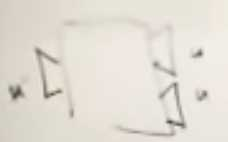
\includegraphics[width=0.8\textwidth]{quantum-cloning-machine}
\end{figure}

\begin{thm}[A quantum cloning machine is impossible]
\end{thm}

\begin{proof}
	 In order to prove that there a quantum cloning machine is impossible, we need merely exhibit one system that cannot be cloned.

	\begin{align*}
		\ket{u}\rightarrow& \ket{u}\ket{u}\\
		\ket{d}\rightarrow& \ket{d}\ket{d}\\
		\ket{r}\rightarrow& \ket{r}\ket{r} \text{, but } \numberthis \label{eq:no:clone:linear}\\
		\ket{r} =& \frac{\ket{u} + \ket{v}}{2} \text{, so linearity tell us}\\
		\frac{\ket{u} +\ket{v}}{2} \rightarrow&  \frac{\ket{u} \ket{u} + \ket{v} \ket{v}}{2} \text{. Does this agree with (\ref{eq:no:clone:linear})? (\ref{eq:no:clone:linear}) gives}\\
		\frac{\ket{u} +\ket{v}}{2}\rightarrow& \frac{\ket{u} +\ket{v}}{2} \frac{\ket{u} +\ket{v}}{2}\\
		\rightarrow& \frac{\ket{u}\ket{u} + \ket{u}\ket{d} + \ket{d}\ket{u}+\ket{d}\ket{d}}{4} 
	\end{align*}

\end{proof}

Our proof exploits the fact that cloning is quadratic, but time evolution is linear, to show that we can build a machine that clones $\ket{u}$ and $\ket{v}$, but not $\ket{r}$. There is some debate about building a machine to clone imperfectly: how good can it be?

\section{Bell's theorem and two-slit experiment}

\subsection{Questions about entanglement}

\begin{enumerate}
	\item What happens if one member of an entangled pair is caught by a black hole? The outside electron becomes entangled with the degrees of freedom of the black hole. When the black hole evaporates, the photons are entangled with the electron that was outside.
	\item What happens if two water molecules become entangled, and then one is placed in a bathtub full of water? The one outside becomes entangled with the state of the bathtub (the entangled molecule in the bathtub gets too mixed up with the others to have a clear identity). So what happens when the bathtub evaporates? The molecule remains entangled with the vapour, unless something comes over from the bathtub to interact with the molecules and break the entanglement. Disentanglement can take place, but only if the systems are close enough to interact.
	\item What happens when we measure two entangled particles? That takes them out. What if we measure only one? It can. These measurements are called "observations", and we'll talk about them during this lecture.
\end{enumerate}

\subsection{Subspaces and Projection Operator}

Review of several topics.
\begin{enumerate}
	\item Duality--bars and kets
	\item Orthogonality
	\item Linear Independence
	\item Dimension
\end{enumerate}

\begin{thm}[Basis vectors]
	In a $D$-dimensional space with orthogonality, we can always find $D$ mutually orthogonal, normalized basis vectors, $\ket{n} n=1,2,...D$.
\end{thm}
\begin{proof}
	TBP
\end{proof}
\begin{thm}[Expansion in basis vectors]
	Any state vector can be written:
	\begin{align*}
		\psi =& \sum_{n=1}^{D} a_n \ket{n} \text{, where}\\
		a_m =& \braket{m\vert\psi} \text{, and}\\
		\psi =& \sum_{n=1}^{D} \ket{n} \braket{n\vert\psi} \numberthis \label{eq:psi_expanded}
	\end{align*}
\end{thm}
\begin{proof}
	TBP
\end{proof}
Introducing the concept or a \emph{dyad}, $\ket{a}\bra{b}$:
\begin{align*}
	\underbrace{\ket{a}\bra{b}}_\text{ A dyad}\psi =& \ket{a}(\bra{b}\psi) \text{, we see from (\ref{eq:psi_expanded}):}\\
	\ket{n}\bra{n} =& I \text{, the "Resolution of the Identity"} \numberthis \label{eq:resolution:identity}
\end{align*}

We will derive some interesting subspaces: subspaces correspond to observable questions that we might ask. Imagine an observable $K$, and consider the eigenvalue/eigenvector:
\begin{align*}
	K \ket{a} =& \lambda \ket{a} \text{ Suppose there is a linearly independent eigenvector with the same eigenvalue}\\
	K \ket{b} =& \lambda \ket{b} \text{, then any linearly independent combination is also an eigenvalue}\\
	K(\alpha \ket{a} + \beta \ket{b}) =& \lambda (\alpha \ket{a} + \beta \ket{b})
\end{align*}

There is a subspace corresponding to the eigenvalue. So the measurement $K=\lambda$ is not necessarily identified with a single vector, but with a subspace. Once you have identified a subspace, you can find a basis. Lets suppose we have found a basis, $\{\ket{a}, \ket{b},...\}$, with dimension $<D$ and construct $\sum_a \ket{a} \bra{a}$

\begin{align*}
	(\sum_a \ket{a} \bra{a}) \psi =& \psi \text{, if $\psi$ in subspace}\\
	=& \text{ projection onto subspace otherwise}\\
	\sum_a \ket{a} \bra{a} =& \mathbb{P}_{K=\lambda} \numberthis \label{eq:projection}
\end{align*}

To construct a projection operator for a value of a property:
\begin{enumerate}
	\item find subspace;
	\item find basis in that subspace;
	\item construct what would have been the identity--(\ref{eq:projection}).
\end{enumerate}
Any projection operator characterizes a property--the property that is true in that subspace.

The probability postulate for quantum mechanics is most nicely expressed in terms of projection operators. Given an arbitrary, normalized, state $\psi$, which may or may not be in the subspace, the probability that $K$ has value $\lambda$ is the expectation: 

\begin{align*}
	\braket{\psi\vert\mathbb{P}_{K=\lambda}\vert\psi}=&\sum_a \braket{\psi\vert a}\braket{a \vert \psi} \text{, e.g.}\\
	\mathbb{P}_\text{first spin up}=&\ket{uu}\bra{uu} + \ket{ud}\bra{ud}
\end{align*}

Two \emph{commuting} projection operators, $\mathbb{P}_{K=\lambda}$ and $\mathbb{P}_{L=\mu}$ enable simple definitions or "and" and "or" (we assume that the subspaces have non-zero vectors in common).

\begin{thm}[Commuting projection operators]\label{thm:commuting}
	If $\mathbb{P}_{K=\lambda}$ and $\mathbb{P}_{L=\mu}$ commute:
	\begin{align*}
		\mathbb{P}_{K=\lambda \land L=\mu} =& \mathbb{P}_{K=\lambda}\mathbb{P}_{L=\mu}\\
		\mathbb{P}_{K=\lambda \lor L=\mu} =& \mathbb{P}_{K=\lambda} + \mathbb{P}_{L=\mu}
	\end{align*}
\end{thm}

\begin{proof}
	\begin{align*}
		K (\mathbb{P}_K\ket{\psi}) =& \lambda (\mathbb{P}_K\ket{\psi}) \text{\because $\mathbb{P}_K\ket{\psi}$ subspace of things with property K}\\
		\mathbb{P}_K\mathbb{P}_L \ket{\psi} =& \mathbb{P}_L\mathbb{P}_K \ket{\psi} \text{, has properties K \& L}
	\end{align*}
	So $\mathbb{P}_K\mathbb{P}_L$ corresponds to K \& L.
\end{proof}

The spin operators for two particles, $\sigma_i$ and $\tau_j$, are compatible.

\subsection{Bell's theorem review}\label{sec:bell:review}

NB: Bell not always violated. It is often true for some properties, not others. LS suggests that you can choose A, B, C so Bell is satisfied, or so that it is not.

In Section \ref{sec:bell}, we saw from (\ref{eq:bell:inequality}), that, for a classical system $$N(A, \neg B) + N(B, \neg C) \ge N(A,\neg C)$$
We consider a two electron system with spins:
\begin{itemize}
	\item A $\uparrow$;
	\item B $\nearrow$;
	\item C $\rightarrow$.
\end{itemize}
Negating a property for one electron is the same as asserting it for the other electron if system is a Singlet. We can recast (\ref{eq:bell:inequality}):
$$N(\uparrow \nearrow) + N(\nearrow \rightarrow) \ge N(\uparrow\rightarrow)$$
Or, in terms of projection operators.
\begin{table}[H]
	\begin{center}
		\caption{Recast (\ref{eq:bell:inequality}) in terms of projection operators, using Theorem \ref{thm:commuting}}
		\begin{tabular}{|c|c|c|} \hline
			$\uparrow\nearrow$&$\nearrow\rightarrow$&$\uparrow\rightarrow$ \\ \hline
			$\frac{1+\sigma_3}{2} \Big(\frac{1+\frac{\tau_1+\tau_3}{\sqrt{2}}}{2}\Big)$&$\Big(\frac{1+\frac{\sigma_1+\sigma_3}{\sqrt{2}}}{2}\Big)\frac{\tau_1+1}{2}$&$\frac{1+\sigma_3}{2} \frac{1+\tau_1}{2}$ \\ \hline
		\end{tabular}
	\end{center}
\end{table}

Question: what sorts of experiment are we describing? Imagine a beam of electrons, which come out in correlated pairs. Electrons in each pair are near each other, they interact, and the lowest energy happens to be the singlet state. After a while they do or don't emit a photon, but they get into the singlet state. Then electrons are taken apart: this isn't hard to do--you send them through some system which separates them. You could use an electron/positron, and use a field to send them their separate ways, so we have many well separated pairs. Now divide into groups so we can do experiments: start with 100 billion pairs, take a third of them and measure $A\land\not B$--we measure the up component of the electron and the $45^{\circ}$ component of the positron, and count how many pairs were $\uparrow\nearrow$. This gives a probability. Repeat for second and third groups, \emph{mutatus mutandi}, to compute the other two probabilities.

When people talk about "non local" mechanisms, they mean that signals have to propagate faster then light.

During the remainder of this lecture we will talk about three things: Interference phenomena; measurement and its connection with entanglement (how a measurement is really the establishment of entanglement between systems); and how measurements destroy interference--the collapse of the wave packet.

\subsection{Two slit and interference} 

Consider an electron that can be in one of 7 positions--Figure \ref{fig:ent-2-slit}. We want the probability that the electron arrives at a particular point in the right hand column.

\begin{figure}[H]
	\begin{center}
		\caption[Two slit experiment]{The two slit experiment. Electron starts in one of 7 positions and moves to the right. When an electron meets the 2nd column it bounces back, unless it is in one of the two positions designated as slits.}\label{fig:ent-2-slit}
		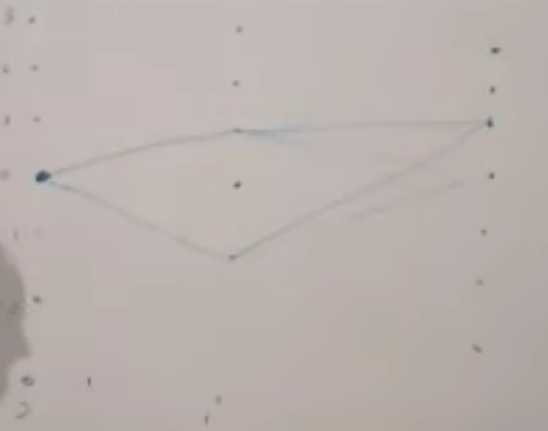
\includegraphics[width=0.8\textwidth]{ent-2-slit}
	\end{center}
\end{figure}
The quantum mechanical evolution of a system is linear. Imagine that a system moves from state $\ket{a}$ to $\ket{a^{\prime}}$ during time $t$, and from  $\ket{b}$ to $\ket{b^{\prime}}$. Then it moves from $\alpha \ket{a} + \beta \ket{b}$ to $\alpha \ket{a^{\prime}} + \beta \ket{b^{\prime}}$ during time $t$.

Electron starts at 0 in first column, and either reaches +1 or -1 in second: by symmetry

\begin{align*}
	\ket{0} \rightarrow& \ket{-1} + \ket{+1}\\
	\ket{+1} \rightarrow& \sum_n \psi_n \ket{n} \text{When electron reaches the 3rd column, "the screen":} \\
	\ket{-1} \rightarrow& \sum_n \phi_n \ket{n} \text{, so, by linearity, after 2 steps starting at $\ket{0}$}\\
	\ket{0} \rightarrow& \sum_n (\psi_n + \phi_n) \ket{n} \text{, so probability for $n$th state is}\\
	(\psi_n^* + \phi_n^*)(\psi_n + \phi_n)=& \underbrace{\psi_n^*\psi_n}_\text{which is all we'd get if we closed first hole} + \psi_n^*\phi_n + \phi_n^*\psi_n + \phi_n^*\phi_n \numberthis \label{eq:P:hole0}
\end{align*}

Classically we'd only get the first and last term, but in quantum mechanics we have the other two as well. By symmetry we might argue that $\psi_0$ and $\phi_0$ should be the same.
\begin{align*}
	\psi_0^*\psi_0 + \psi_0^*\phi_0 + \phi_0^*\psi_0 + \phi_0^*\phi_0 =& 4\psi_0^*\psi_0\numberthis \label{eq:constructive:interferance}
\end{align*}
This is 4 times the probability that we'd get if $-1$ blocked; classically we'd expect 2 times!
Figure \ref{fig:change:sign}, however,  depicts an apparatus that changes the sign in the wave function, so  $\ket{0} \rightarrow \ket{-1} - \ket{+1}$. Now the terms in (\ref{eq:constructive:interferance}) cancel, giving destructive interference. The electron can get to a position either via the upper route or lower, but, if you open up both routes, it is impossible to get through! This is as odd as the Bell inequality. Probabilities in quantum mechanics are not doing what they do in classical mechanics: the probabilities for exclusive outcomes don't add; the \emph{amplitudes} add.

\begin{figure}[H]
	\begin{center}
		\caption{Apparatus to change sign $\ket{0} \rightarrow \ket{-1} - \ket{+1}$}\label{fig:change:sign}
		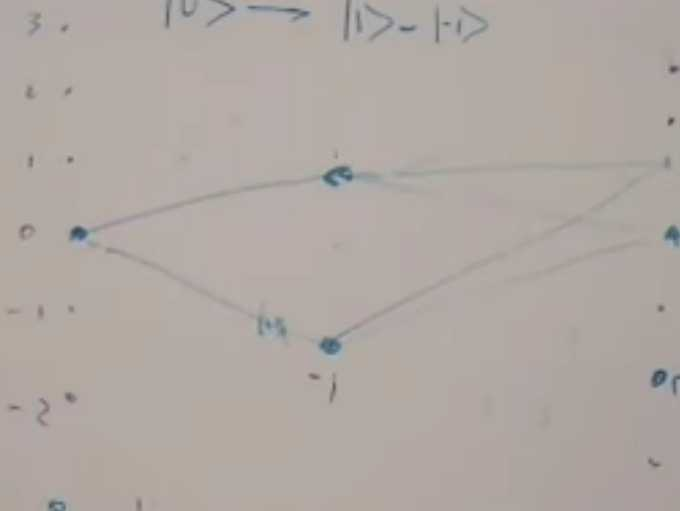
\includegraphics[width=0.8\textwidth]{ent-2-slit-change-sign}
	\end{center}
\end{figure}

\subsection{Measurement \& entanglement in the 2 slit experiment}

What happens if there is an apparatus that monitors--measures and records--which slit the electron goes through? In QM we can't do arbitrarily gentle experiments. It turns out we will change answers in a dramatic way and destroy interference. The electron becomes entangled with the apparatus.

Place a spin next to the upper hole, initially down. If electron passes through upper hole, spin flips up, otherwise it stays down. System starts at $\ket{0,d}$. If we close lower hole we get $\ket{+1,u}$; closing upper hole gives $\ket{-1,d}$. Opening both gives $\ket{+1,u}+\ket{-1,d}$: the electron and spin have become entangled. What happens at screen? Assume spin is unaffected.

\begin{align*}
	\ket{+1,u} \rightarrow& \sum_n \psi_n \ket{n,u}  \\
	\ket{-1,d} \rightarrow& \sum_n \phi_n \ket{n,d} \\
	\ket{0} \rightarrow& \sum_n \big(\psi_n \ket{n,u} + \phi_n \ket{n,d}\big)
\end{align*}

If we try to compute the probability of the electron going through hole 0 in the screen, we no longer have the cross terms from (\ref{eq:P:hole0}), since $\braket{u\vert d}=0$.

Making a measurement is establishing entanglement between the device and the system. The destruction of the interference is what is known as the "collapse of the wave function".

Can't electron become entangled with an atom in the surround to the slit? Yes, and that destroys the interference pattern. Photons are easier, as they don't interact so much. Electric field of electron may interact with something: if the disturbance is enough that you can tell which slit the electron went through, then you completely destroy the interference pattern. \begin{itemize}
	\item If electron moves the probability distribution of some degree of freedom enough that you know which slit it went through, then you lose interference.
	\item If it shifts just a little bit, so you don't know which slit, then interference will not be completely destroyed.
\end{itemize}

It is a matter of degree: freeze things, put everything into ground state, so nothing is easily disturbed; then you can create pretty much the idealized situation where, after you have gone through, there is nothing that has been recorded. If there is an energy gap, and the photon/electron has low energy, it might not be able to make the disturbance: so you have the interference pattern.

NB: an experiment either means many repetition, or many particles. You need statistics to see the probabilities.


\section{Measurement, Entropy, the Density Matrix}

\subsection{Two slit interference and measurement} 
LS reviewed the two slit experiment, replacing $\{+1,-1\}$ with $\{A,B\}$. He notes that classically the probabilities add: to get the probability for a point on the screen with both slits open is the sum of the probabilities with $A$ (only) open, and $B$ (only open.) 

\begin{align*}
	\ket{0}\rightarrow& \ket{A} + \ket{B}\\
	\ket{A} \rightarrow& \sum_n \psi_n \ket{n}\\
	\ket{B} \rightarrow& \sum_n \phi_n \ket{n}\\
	P_n^A =& \psi_n^* \psi_n\\
	P_n^B =& \phi_n^* \phi_n\\
	\ket{A} + \ket{B} \rightarrow & \sum_n \big(\psi_n + \phi_n\big) \ket{n}\\
	P_n^{A+B} =& \big(\psi_n^* + \phi_n^*\big)\big(\psi_n + \phi_n\big)\\
	=& \underbrace{\psi_n^*\psi_n + \phi_n^*\phi_n}_\text{sum of original probabilities} + \underbrace{\phi_n^*\psi_n + \psi_n^*\phi_n}_\text{interference term}
\end{align*}

$P_n^{A+B}$ gives twice classical probability, other positions give zero.

What happens if someone watches whether electron goes through one hole or the other? In the previous lecture we used a spin to record whether the electron went through A.
\begin{align*}
	\ket{0,d}\rightarrow& \ket{A,u} + \ket{B,d} \text{, states correlated and entangled}\\
	\ket{A,u} \rightarrow& \sum_n \psi_n \ket{n,u}\\
	\ket{B,d} \rightarrow& \sum_n \phi_n \ket{n,u} \numberthis \label{eq:twin:slit:AB}
\end{align*}
Terminology:
\begin{itemize}
	\item "collapsing the wavepacket" is the language to use if you don't want to remember the extra spin--collapse to $A$ or $B$;
	\item "establishment of entanglement" is used when we keep the apparatus in our description.
\end{itemize}
What if particle gives a little kick to the screen, sufficient for us to know which hole it went through? Screen has an uncertainty in its momentum because it is well localized. particle shifts distribution, but slightly, so we don't get precise information concerning the hole.

Now, suppose that we do establish the entanglement of (\ref{eq:twin:slit:AB}), and calculate the probability of the electron being found at point $m$. There are two ways this can happen: with spin up, or spin down. We need to build the projection operator for being found at point $m$. So for $A+B$ we have:

\begin{align*}
	\sum_n&\big(\psi_n^* \bra{n,u}+\phi_n^*\bra{n,d}\big)\big(\ket{m,u}\bra{m,u} + \ket{m,d}\big)\ket{m,d} \sum_n\big(\psi_n \ket{n,u}+\phi_n\ket{n,d}\big)\\
	=& \psi_m^* \psi_m +\phi_m^* \phi_m \text{. Cross terms vanish because of orthogonality.}
\end{align*}

So if you do an experiment, probabilities sum as in classical physics.

\subsubsection{High energy electrons emitting photons and destroying interference without explicit measurement} 

\begin{itemize}
	\item The problem is not the spin, it is the correlation between the spin and the path. An additional "up" on both paths would not cancel interference.
	\item LS doesn't need to look at the spin: it is enough that the path has been recorded to destroy interference.
	\item When electron is accelerated it may emit a photon, with a probability of 0.01 for a slowly moving electron. You cannot be certain which hole it went through. If the energy is really high, likelihood of emitting a photon is much higher, so interference may be partially destroyed. So the ability to emit photons may partially destroy interference pattern. 
	\item If you know that probability is not quite 50-50, interference is destroyed a little bit.
	\item The atmosphere is a source of interference.
	\item Moon doesn't appear fuzzy, partly because it is heavy, partly because it is being constantly bombarded (observation).
\end{itemize}

Key take home: \begin{itemize}
	\item if anything tags the electron so we know which part it went interference will be destroyed;
	\item if we only know probabilities for each hole, interference will be partially destroyed.
\end{itemize}

\subsubsection{Schr\"odinger's cat and Wigner's friend}

Schr\"odinger's cat is \emph{not} in a superposition of alive and dead. The cat is entangled: it is part of an entangled system.
\begin{itemize}
	\item Start with a live cat, and an unfired gun, $\ket{lu}\rightarrow\alpha\ket{lu}+\beta\ket{df}$
	\item You can not do an interference experiment with live and dead.
	\item You don't have to look at the cat to determine whether it is alive or dead, you can look at the gun.
\end{itemize}

We can't talk about the electron having been at A or B unless we measure it: electron has to do something that it has arrived. We also to an experiment at the screen to record the fact that the electron has arrived (E.g. we don't look at the electron, we look at the black spot on a photographic plate, which has become entangled with the electron).

The process of separating a system into that which measures, and that which is measured is always ambiguous. We can say that the experiment doesn't complete until "I" look at the spin, in which case we add another element, "me"; this has two states, having seen spin up, and recorded that in my brain, and having seen and recorded down ($\ket{A,up,up}$). But someone else could be observing me: we'd still have consistency. Schr\"odinger opens box, and he becomes entangled, then Wigner asks Schr\"odinger what he saw,...

\subsection{Entropy, level of entanglement}  

How do you define a measure of entanglement? Entanglement Entropy does this.

What is classical entropy? Entropy is a property of the system and my state of knowledge abut the system. The less I know about the system the more the entropy. Imagine a classical system with $N$ states, where we know that the system is in one of $n$ states with equal probability. We can say that our degree of ignorance is $n$. If $n=1$, we say entropy is zero. If $n=N$, we know nothing about which state the system is in--maximum entropy.
\begin{defn}[Entropy]
	\begin{align*}
		S=&\log{n}\text{, or, more generally}\\
		S =&- \sum_i P_i \log{P_i}
	\end{align*}
\end{defn}

The difference between actual entropy and maximum entropy is called "information".

\subsection{Trace and Density matrix }

Let $M$ be a matrix/linear operator in a space with basis $\ket{i}$ and consider the trace:
\begin{align*}
	\Tr M =& \sum_i \braket{i\vert M \vert i}
\end{align*}

\begin{thm}[The trace of a matrix is the negative sum of its eigenvalues]\label{thm:sum:ev}
	\begin{align*}
		\Tr A =& - \sum_i \lambda_i \text{, where we count degenerate eigenvalues in accordance with their multiplicity.}
	\end{align*}
\end{thm}

\begin{proof}
	See Appendix \ref{proof:sum_ev}
\end{proof}

\begin{cor}[The trace of a matrix is independent of the choice of basis]\end{cor}
\begin{proof}
	From Theorem \ref{thm:sum:ev} $\Tr A = - \sum_i \lambda_i$, but the eigenvalues are independent of the choice of basis.
\end{proof}

Now if M is Hermitian,there is a basis in which the matrix is diagonal, so the trace is the sum of the eigenvalues.

\begin{align*}
	\bar{F} =& \sum_i P_i F_i \text{Classical expected value}\\
	\sum \rightarrow& \Tr \text{, in passage to quantum mechanics}
\end{align*}
Imagine that someone creates a system in a state $\ket{i}$, but they only tell us the probability distribution, $\rho_i$. We define the density matrix, the analogue of the classical $P_i$:
\begin{defn}[The density matrix, $\rho$]
	\begin{align*}
		\begin{pmatrix}
			\rho_1&0&0&0&...\\
			0&\rho_2&0&0&...\\
			0&0&\rho_3&0&...\\
			0&0&0&\rho_4&...\\
			0&0&0&0&...
		\end{pmatrix}
	\end{align*}
\end{defn}
The trace of the density matrix is 1.
We have an observable $F$. If we were in the $i$th state, the expectation would be $\braket{i\vert F \vert i}$.
\begin{thm}[$\bar{F}= \Tr F \rho$.]
	i.e. in the case where all we know is the $\rho_i$
\end{thm}
\begin{proof}
	\begin{align*}
		\Tr F \rho=&\sum_i \braket{i \vert F \rho \vert i}\\
		=& \sum_{i,j} \braket{i \vert F \vert j} \braket{j \vert \rho \vert i} \text{, from (\ref{eq:resolution:identity}) "resolution of the identity"}\\
		=& \underbrace{\sum_i \braket{i \vert F \vert i}}_\text{Expectation if in state $i$} \underbrace{\rho_i}_\text{Probability of being in state i}\\
		=& \bar{F}
	\end{align*}
\end{proof}

\begin{thm}[$\Tr(AB)=\Tr(BA)$]This is true even if the two matrices don't commute.
\end{thm}
\begin{proof}
	\begin{align*}
		\Tr AB =& \sum_i (AB)_{ii} \text{, by definition of trace}\\
		=& \sum_{i,j} a_{ij} b_{ij} \text{, by definition of matrix multiplication}\\
		=& \sum_{i,j} b_{ij} a_{ij} \text{, on rearranging}\\
		=& \sum_i (AB)_{ji} \text{, by definition of matrix multiplication}\\
		=& \Tr BA \text{, by definition of trace}
	\end{align*}
\end{proof}
We now introduce the quantum mechanical definition of entropy. If one $rho_i$ is 1 and all the others zero, entropy is zero.

\begin{align*}
	S =& -\Tr \rho \log{\rho}
\end{align*}


\section{Entropy \& Dynamics}

\subsection{Entropy and Density matrix; Measuring Entanglement Entropy} 

\begin{itemize}
	\item The density matrix is more general than the state vector, as it incorporates information about how the system was prepared. 
	\item If you know nothing, density matrix is $\frac{1}{N}I$: all possibilities are equally weighted.
	\item Density matrix has all eigenvalues real and non-negative $\lambda_i,\; i=1,2,...N$. The eigenvectors form an orthonormal basis.
	\item  The probability of having been prepared in the state corresponding to the $i$th eigenvector is $\lambda_i$.
	\item Extremes of knowledge are $\frac{1}{N}I$ and a pure state $\ket{\psi}$: density matrix if projection onto that pure state $\ket{\psi} \bra{\psi}$. 
\end{itemize}

Consider an observable $M$ for a system in a pure state $\ket{\psi}$:
\begin{align*}
	\bar{M} =& \Tr \rho M\\
	=& \sum_i \braket{i \vert \rho M \vert i}\\
	=& \sum_i \braket{i \vert \psi}\braket{\psi \vert M i}\\
	=& \sum_i \braket{\psi \vert M i} \braket{i \vert \psi}\\
	=& \braket{\psi \vert M \psi} \; \because \sum_i \ket{i}\bra{i}=I
\end{align*}

This isn't surprising for a pure state. Suppose that we don't have a pure state.
\begin{align*}
	\bar{M} =& \Tr \rho M\\
	=& \sum_i \braket{i \vert \rho M \vert i} \\
	=& \sum_{i,j} \braket{i\vert\rho j} \braket{j\vert M \vert i}\\
	=& \sum_j \lambda_j \braket{j\vert M \vert j} \text{, in the basis in which $\rho$ is diagonal}
\end{align*}

Entanglement happens when we have more than one system. Let's suppose we have a system composed of two parts, and suppose we have a basis labelled $\ket{ab}, a \in [1,N], b \in [1,n]$. The most general state is $\sum_{a,b}\psi(a,b)\ket{ab}$ where $\sum_{a,b}\psi(a,b)^*\psi(a,b)=1$

Suppose we do an experiment that doesn't involve $b$. Alice measures observable $M$ so A.

\begin{align*}
	\bar{M}=&\sum_{a,b,a^{\prime},b^{\prime}}\psi^*(a^{\prime},b^{\prime})\braket{a^{\prime}b^{\prime}\vert M \vert ab} \psi(a,b)\\
	=&\sum_{a,b,a^{\prime}}\psi^*(a^{\prime},b)\braket{a^{\prime}b\vert M \vert ab} \psi(a,b) \text{$\because$ $M$ acts only on $A$.}\\
	=& \sum_{a,a^{\prime}}  M_{a,a^\prime} \sum_b \psi^*(a^{\prime},b) \psi(a,b)\\
	=& \sum_{a,a^{\prime}}  M_{a,a^\prime} \rho_{a,a^\prime}\\
	=& \Tr M \rho
\end{align*} 



\subsection{Subsystems in pure states}
When does $\psi(a,b)$ represent subsystems that are in pure states? When it factorizes into separate functions of $a$ and $b$--$\psi(a,b)=\phi(a) \chi(b)$. We'll compute the density matrix.

\begin{align*}
	\rho_{ab} =& \sum_b \phi(a) \chi(b) \phi^*(a^\prime) \chi^*(b)\\
	=& \phi(a) \phi^*(a^\prime) \underbrace{\sum_b  \chi(b)  \chi^*(b)}_\text{=1}\\
	=& \phi(a) \phi^*(a^\prime) \text{, then the expectation of the observable $M$ is}\\
	\bar{M} =& \sum_{a,b}\phi(a) M_{a,a^\prime}\phi^*(a^\prime)\\
	=& \braket{\phi\vert M\vert \phi}
\end{align*}
$b$ can be ignored, and we can describe using a pure state $a$. But most functions aren't products! If entropy is small we are close to a product, if large we are entangled.

We illustrate with two examples.

\subsubsection{The Singlet}

\begin{align*}
	&\frac{\ket{ud}-\ket{du}}{\sqrt{2}} \text{. We express as a wave function}\\
	\psi(u,u) =& 0\\
	\psi(u,d) =& \frac{1}{\sqrt{2}}\\
	\psi(d,u) =& \frac{1}{\sqrt{2}}\\
	\psi(d,d) =& 0
\end{align*}

We calculate the density matrix for the $A$ system, the first spin.
\begin{align*}
	\rho_{uu} =& \psi(u,u)\psi^*(u,u) +  \psi(u,d)\psi^*(u,d) =& \frac{1}{2}\\
	\rho_{ud} =& \psi(u,u)\psi^*(d,u) +  \psi(u,d)\psi^*(d,d) =& 0\\
	\rho_{du} =& \psi(d,u)\psi^*(u,u) +  \psi(d,d)\psi^*(u,d) =& 0\\
	\rho_{dd} =& \psi(d,u)\psi^*(d,u) +  \psi(d,d)\psi^*(d,d) =& \frac{1}{2}
\end{align*}

\begin{align*}
	\rho =& \begin{pmatrix}
		\frac{1} {2}&0\\
		0 &\frac{1}{2}
	\end{pmatrix}
\end{align*}
Entropy is $\log{2}$: maximum value - complete ignorance.

What is expectation of spin?

\begin{align*}
	\vec{\sigma} \cdot \vec{\hat{n}} =& \Tr \rho \sigma \cdot n\\
	=& \Tr \frac{1}{2} I \sigma \cdot n\\
	=& \frac{1}{2} \Tr\sigma \cdot n\\
	=& 0
\end{align*}

Singlet is maximally mixed state.

\subsubsection{Another example: not the Singlet}
Consider:
\begin{align*}
	\psi(u,u) =& \frac{1}{2}\\
	\psi(u,d) =& \frac{1}{2}\\
	\psi(d,u) =& \frac{1}{2}\\
	\psi(d,d) =& \frac{1}{2} \text{, then}\\
	\rho_{uu} =& \frac{1}{4} \\
	\rho_{ud} =& \frac{1}{4}\\
	\rho_{du} =&  \frac{1}{4}\\
	\rho_{dd} =&  \frac{1}{4} \text{, i.e.}\\
	\rho =& \begin{pmatrix}
		\frac{1} {2}&\frac{1} {2}\\
		\frac{1} {2} &\frac{1}{2}
	\end{pmatrix}	
\end{align*}
We'll calculate the eigenvalues.
\begin{thm}[Product and sum of eigenvalues]
	For a matrix $A$ with eigenvalues  $\{\lambda_i\}$:
	\begin{align*}
		\prod_i \lambda_i =& \vert A \vert \text{ Product of eigenvalues = determinant} \numberthis \label{eq:prod:ev}\\
		\sum_i \lambda_i =& \Tr A \text{ Sum of eigenvalue=trace} \numberthis \label{eq:sum:ev}
	\end{align*}
\end{thm}
\begin{proof}
	\begin{enumerate}
		\item \eqref{eq:sum:ev} is proved in Section \ref{proof:sum_ev}, as part of proving Theorem \ref{thm:sum:ev}
		\item \eqref{eq:prod:ev} can be seen as an application of the last of Vi\`ete's  formulae\cite{enwiki:1030161470}.
	\end{enumerate}
\end{proof}
So we know eigenvalues are 0 and 1; entropy is zero. This is a product state.

\begin{align*}
	\Tr \rho \sigma_3 =& 0\\
	\Tr \rho \sigma_1 =& 1
\end{align*}

A pair of spins along the x-axis!

The entropy that is exhibited in these examples is called \emph{entanglement entropy}. 



\subsubsection{Entropy is not additive}

NB: we are talking about entropy of a subsystem, not the combined system, which had zero entropy. Entropy in general does not add; in particular entanglement entropy does not add.

\subsection{Dynamics in time - Schr\"odinger equation}

In classical logic, if we are dealing with a discrete system, the only thing that makes sense is discrete time, and we permute points in configuration space. In quantum mechanics, we can have discrete systems, but evolution can be continuous.

Assumption: the logical relationship between states does not change with time. Two orthogonal states will evolve into orthogonal states. The inner product between states remains the same.

Actually, this is second principle: linearity is first.


\subsubsection{Unitary operators}\label{sect:unitary}

Start with system in state $\ket{\psi(0)}$ and evolves to $\ket{\psi(t)}$

\begin{align*}
	\ket{\psi(t)} =& U(t) \ket{\psi(0)} \text{, where} \numberthis \label{eq:evolution_time}\\
	U(0) =& I\\
	\braket{\psi(t)\vert\phi(t)} =& \braket{\psi(0)\vert\phi(0)} \text{, as stated above.}\\
	\bra{\phi(t)} =& \bra{\phi(0)} U^\dagger(t) \text{, whence}\\
	\braket{\psi(t)\vert\phi(t)} =& \braket{\psi(0)\vert U^\dagger(t) U(t)\vert\phi(0)}\\
	=& \braket{\psi(0)\vert\phi(0)} \\
	=& \braket{\psi(0)\vert I \vert \phi(0)} \text{, so we can show}\\
	 U^\dagger(t) U(t)=& I \text {, Unitary!}
\end{align*}

\subsubsection{Hamiltonian}

Imagine a very small time evolution $t=\epsilon$, where $\epsilon^2$ can be ignored.

\begin{align*}
	U(\epsilon) =& 1 - i \epsilon H \numberthis \label{eq:introducing:hamiltonian}\\
	U^\dagger (\epsilon) =& \\
	U^\dagger (\epsilon)U(\epsilon) =& \big(1 + i \epsilon H^\dagger\big)\big(1 - i \epsilon H\big)\\
	=& I + i\epsilon (H^\dagger-H) + O(\epsilon^2) \text{, which must equal I for Unitarity}\\
	H^\dagger=& H \text{, unitarity of $U\implies$ $H$ is Hermitian}
\end{align*}

\begin{itemize}
	\item $H$ must be Hermitian; it is called the Hamiltonian.
	\item $H$ is an observable, the Energy.
	\item The eigenvalues of $H$ are the energy levels.
\end{itemize}
Writing the foregoing differently:
\begin{align*}
	\ket{\psi(\epsilon)} - \ket{\psi(0)} =& -i \epsilon H \ket{\psi(0)}\\
	\frac{\ket{\psi(\epsilon)} - \ket{\psi(0)}}{\epsilon H } =& -i \ket{\psi(0)}\\
	\frac{\partial \ket{\psi}}{\partial t} =& -\frac{i}{\hbar}  H \ket{\psi} \text{, Schr\"odinger's equation} \numberthis \label{eq:schroedinger}
\end{align*}

We have introduced Planck's constant.

Now let us consider an eigenvalue/eigenvector. Assume $\ket{\psi}$ remains an eigenvector for all time:
\begin{align*}
	H \ket{\psi} =& E \ket{\psi} \\
	\ket{\psi(t)} =& f(t) \ket{\psi(0)}\\
	\frac{\partial f}{\partial t} =&-i \frac{E}{\hbar}f\text{, whence}\\
	f(t) =& e^{-i \frac{E}{\hbar} t}
\end{align*}
So an eigenvector evolves with time by multiplying by a time-dependent phase. Angular frequency is $\frac{E}{\hbar}$.


\section{Hamiltonian}

\subsection{Dynamics of states in time; Hamiltonian is Energy}
In the previous lecture we looked at how systems change with time. The state of a system is described by a ket vector, $\ket{\psi}$, which moves around with time. The rule is it moves under the influence of a linear operator--(\ref{eq:evolution_time}). The assumption that evolution is linear cannot be proved: it is a postulate that is rooted in experiment, plus the fact that everyone who has tried to change it has ended up with conceptual difficulties, such as energy not being conserved, probability is not defined, etc. We expect probability to be conserved.

\begin{thm}[Conservation of probability requires the inner product of any two vectors to be independent of time]
	\begin{align*}
		\braket{\psi(t)\vert \psi(t)} =& \braket{\psi(0)\vert \psi()} \text{, $\forall t, \psi()$}\\
		\implies&\\
		\braket{\phi(t)\vert \psi(t)} =& \braket{\phi(0)\vert \psi()} \text{, $\forall t, \psi(), \phi()$}
	\end{align*}
\end{thm}
\begin{proof}
	TBP
\end{proof}
\begin{defn}[Unitarity]
	If $U^\dagger U=1$, we say that $U$ is unitary.
\end{defn}

\begin{thm}[The matrix describing the evolution of the wave function (\ref{eq:evolution_time}) is unitary]
\end{thm}
\begin{proof}
	\begin{align*}
		\ket{\psi(t)} =& U(t) \ket{\psi(0)} \text{, where} \\
		U(0) =& I\\
		\braket{\psi(t)\vert\phi(t)} =& \braket{\psi(0)\vert\phi(0)} \text{, as stated above.}\\
		\bra{\phi(t)} =& \bra{\phi(0)} U^\dagger(t) \text{, whence}\\
		\braket{\psi(t)\vert\phi(t)} =& \braket{\psi(0)\vert U^\dagger(t) U(t)\vert\phi(0)}\\
		=& \braket{\psi(0)\vert\phi(0)} \\
		=& \braket{\psi(0)\vert I \vert \phi(0)} \text{, so we can show}\\
		U^\dagger(t) U(t)=& I \text {, Unitary!}
	\end{align*}
\end{proof}

Why is Planck's constant so small? Why is Avogadro's number so large? This aren't questions about physics, but about human biology.

\begin{thm}[In (\ref{eq:introducing:hamiltonian}),  unitarity of $U\implies H$ is Hermitian]
\end{thm}
\begin{proof}
	RB{content...}
\end{proof}

So $H$ is an observable: every system must an $H$, otherwise it could not evolve. It is, of course, the Hamiltonian (as an operator): its eigenvalues are called Energy levels.

What is energy? Force times distance doesn't help us the understand the energy of the electromagnetic field.  We need a more general definition. One way to characterize energy is that it is conserved: that is the single most important thing about it. For certain familiar systems it takes a certain form.

Another definition of Energy:
$$E = h\nu = \hbar \omega$$
What is the connection between this $E$ and the $H$ in the Schr\"odinger equation, (\ref{eq:schroedinger})? Since $H$ is Hermitian it has a complete set of eigenvectors, which we will use as a basis. Note that an eigenvector remains an eigenvector, since we are adding a little vector proportional to it and to $\epsilon$.

\begin{align*}
	H\ket{\psi_E} =& E\ket{\psi_E}\text{, let us try:}\\
	\ket{\psi_E(t)} =& f(t)\ket{\psi_E}\\
	\dot{f}\ket{\psi_E} =& -\frac{iH}{\hbar}\ket{\psi_E}\\
	=& -\frac{iE}{\hbar} f(t) \ket{\psi_E}\\
	\dot{f}=& -\frac{iE}{\hbar} f\\
	f(t) =& e^{-\frac{iE}{\hbar}t}\\
	=& e^{-i \omega t} \text{, see definition of energy in terms of $\omega$}
\end{align*}

What if we have a vector that is a sum of eigenvectors. Any vector can be so expanded. What happens to $\sum_n \alpha_n \ket{\psi_n}$ with time?

\begin{align*}
	\sum_n \alpha_n \ket{\psi_n} \rightarrow \sum_n \alpha_n e^{-\frac{iE_n}{\hbar}t} \ket{\psi_n}
\end{align*}

How do other observables change with time? How do their expectations change with time?

\begin{align*}
	\bar{A} =&\braket{\psi\vert A \psi}\text{. We want to compute}\\
	\frac{\bar{A}}{dt} =&	\braket{\dot{\psi}\vert A \psi} + \braket{\psi\vert A \dot{\psi}} \text{, since $A$ constant}\\
	=& \frac{i}{\hbar}\braket{\psi\vert H A \psi} - \frac{i}{\hbar}\braket{\psi\vert A H \psi}\\
	=& \frac{i}{\hbar} \braket{\psi \vert \big(HA-AH\big)\vert \psi}\\
	=& \frac{i}{\hbar} \braket{\psi \vert \big[H,A\big]\vert \psi} \text {, commutator} \numberthis \label{eq:evolve:state}
\end{align*}

\subsection{Commutators and conservation}

From the foregoing $\dot{\bar{A}} = \bar{\big[H,A\big]}$. That is the fundamental significance of the Hamiltonian. Clearly $\dot{\bar{H}} = \bar{\big[H,H\big]} = 0$.

The set of things that commute with the Hamiltonian is the set of conserved quantities.

\subsection{Mixed state of energy}

The Hamiltonian is Hermitian, so it has a complete set of eigenvectors. If you use this as the basis, $H$ is diagonal. $U$ is also diagonal, with exponentiation. $U = e^{-i\frac{H}{\hbar}t}$

Combine two non-interacting systems: energies (and, hence, frequencies) add.

\subsection{Spin in a magnetic field}

We have $\sigma_1$, $\sigma_2$, $\sigma_3$ and the magnetic field, $\vec{B}$. Magnetic moment is proportional to spin: $\vec{mu} = \frac{\mu}{2}\sigma$, and $E=\frac{\mu}{2}\sigma \cdot \vec{B}.$

\begin{align*}
	H =& \frac{\mu}{2}\sigma \cdot \vec{B}\\
	=& \frac{\mu}{2}\sigma_3 B \text{, if we align the magnetic field with z-axis}
\end{align*}

We compute the time derivative of expected spins.
\begin{align*}
	\dot{\sigma_3} =& \frac{i}{\hbar} \big[H,\sigma_3\big]\\
	\propto& [\sigma_3,\sigma_3] \\
	=& 0\\
	\dot{\sigma_1} =& \frac{i}{\hbar} \big[H,\sigma_1\big]\\
	=& \frac{i}{\hbar} \frac{\mu}{2} B \big[\sigma_3,\sigma_1\big]\\
	=& \frac{i}{\hbar} \frac{\mu}{2} B 2 i \sigma_2\\
	=& - \frac{\mu B}{\hbar} \sigma_2\\
	\dot{\sigma_2} =&  \frac{\mu B}{\hbar} \sigma_1
\end{align*}
We have a point rotating in a plane.
\begin{align*}
	\sigma_1 = \cos{\frac{\mu B}{\hbar} t}\\
	\sigma_2 = \sin{\frac{\mu B}{\hbar} t}
\end{align*}


\subsection{Singlet vs Triplet states}

Two electrons providing fields for each other:
\begin{align*}
	H \propto \vec{\sigma} \cdot \vec{\tau}
\end{align*}
\begin{thm}	[$H \propto \vec{\sigma} \cdot \vec{\tau}$ has 4 eigenvectors: singlet and triplet(degenerate)]
	Let $\alpha_{uu}\ket{uu} + \alpha_{ud}\ket{ud} +\alpha_{du}\ket{du} + \alpha_{dd}\ket{dd}$ be an eigenvector of $\vec{\sigma} \cdot \vec{\tau}$ with eigenvalue $E$.
	\begin{align*}
		\big(\sigma_1\tau_1 +& \sigma_2\tau_2 + \sigma_3\tau_3\big) \big(\alpha_{uu}\ket{uu} + 	\alpha_{ud}\ket{ud} +\alpha_{du}\ket{du} + \alpha_{dd}\ket{dd}\big) \\=& E \big(\alpha_{uu}\ket{uu} + \alpha_{ud}\ket{ud} +\alpha_{du}\ket{du} + \alpha_{dd}\ket{dd}\big) \numberthis \label{eq:ev_sigma_tau} \text{, where}\\
		1 =& \alpha_{uu}^2 + \alpha_{ud}^2 +\alpha_{du}^2 + \alpha_{dd}^2 \numberthis \label{eq:norm:alpha}
	\end{align*}
Then there are two eigenvalues, $+1$ and $-3$. The first eigenvalue corresponds to the singlet, and the other is degenerate, giving rise to the triplet.
\end{thm}

\begin{proof}
 	The left hand side of \eqref{eq:ev_sigma_tau} expands to:
	\begin{align*}
		& \alpha_{uu}\big(\ket{dd} - \ket{dd} + \ket{uu}\big) + \alpha_{ud}\big(\ket{du} +\ket{du} - \ket{ud}\big)\\
		&+\alpha_{du}\big(\ket{ud} +\ket{ud} - \ket{du}\big) + \alpha_{dd}\big(-\ket{uu} + \ket{uu} +\ket{dd}\big)\\
		=&  \alpha_{uu} \ket{uu} + \big( 2 \alpha_{du} - \alpha_{ud}\big)\ket{ud} + \big( 2 \alpha_{ud} - \alpha_{du} \big)\ket{du}+ \alpha_{dd}\ket{dd}	
	\end{align*}
	Equating with the RHS of (\ref{eq:ev_sigma_tau}):
	\begin{align*}
		\alpha_{uu} =& E \alpha_{uu} \numberthis \label{eq:alpha:uu}\\
		 2 \alpha_{du} - \alpha_{ud} =& E \alpha_{ud} \text{, or, rearranging}\\
		  2 \alpha_{du} =& (1+E) \alpha_{ud} \numberthis \label{eq:alpha:ud}\\
		 2 \alpha_{ud} - \alpha_{du}=& E \alpha_{du}\text{, or, rearranging}\\
		 2 \alpha_{ud} =& (1+E)\alpha_{du} \numberthis \label{eq:alpha:du}\\
		 \alpha_{dd} =& E \alpha_{dd} \numberthis \label{eq:alpha:dd}
	\end{align*}

   \eqref{eq:alpha:ud} and \eqref{eq:alpha:du} imply:
   \begin{align*}
   	4 \alpha_{du} =& (1+E)\big(2\alpha_{ud}\big)\\
   	=& (1+E)^2 \alpha_{du} \text{, whence}\\
   	E+1 =& \pm 2 \text{, (unless $\alpha_{du}=\alpha_{ud}=0$)}\\
   	E =& 1 \text{, or}\\
   	 =& -3
   \end{align*}
	We will consider each value in turn.
	\begin{align}
		E =& -3\\
		\implies &\\
		\alpha_{uu} =0 \land& \alpha_{dd}= 0 \text{, from \eqref{eq:alpha:uu} and \eqref{eq:alpha:dd}. Moreover }\\
		\alpha_{du} =& - \alpha_{ud} \text{, from \eqref{eq:alpha:ud} and \eqref{eq:alpha:du}}
	\end{align}
	Using \eqref{eq:norm:alpha}, the values are unique modulo a phase. This is the singlet.
	\begin{align*}
		\frac{1}{\sqrt{2}}\big(\ket{ud}-\ket{du}\big)
	\end{align*}
	Since we are working in a 4-dimensional space, spanned by $\{\ket{uu}, \ket{ud}, \ket{du}, \ket{dd}\}$, and $\vec{\sigma}.\vec{\tau}$ is Hermitian, it is possible to find a basis of 4 eigenvectors; $E=1$ must be degenerate, and be associated with 3 independent eigenvectors.
	It is clear that this eigenvalue imposes no constraints on $\alpha_{uu}$ or $\alpha_{dd}$-- \eqref{eq:alpha:uu} and \eqref{eq:alpha:dd}; moreover $\alpha_{du} = \alpha_{ud}$  from \eqref{eq:alpha:ud} and \eqref{eq:alpha:du}. We can easily choose three eigenvalues, which correspond to the triplet state--Table \ref{eq:basis3}.
	\begin{table}[H]
		\caption{Three independent eigenvectors for $E=1$}\label{eq:basis3}
		\begin{center}
			\begin{tabular}{|r|r|r|r|}\hline
			$\alpha_{uu}$& $\alpha_{ud}$&$\alpha_{du}$&$\alpha_{dd}$\\ \hline
			$\frac{1}{\sqrt{2}}$&0&0&$\frac{1}{\sqrt{2}}$\\ \hline
			0&$\frac{1}{\sqrt{2}}$&$\frac{1}{\sqrt{2}}$&0\\ \hline
			$\frac{1}{\sqrt{2}}$&0&0&$-\frac{1}{\sqrt{2}}$\\ \hline
		\end{tabular}
		\end{center}
	\end{table}

\end{proof}

Given an initial state, we can determine its evolution as follows:
\begin{enumerate}
	\item expand in eigenvectors,
	\item evolve using \eqref{eq:evolve:state},
	\item disentangle to original basis.
\end{enumerate} 

Suppose we start the system as $\ket{ud}$. We will expand in eigenvectors.
\begin{align*}
	\ket{ud} =& \frac{\ket{ud}+\ket{du}}{\sqrt{2} \sqrt{2}} + \frac{\ket{ud}-\ket{du}}{\sqrt{2} \sqrt{2}}\\
	=& \frac{\ket{T}}{\sqrt{2}} + \frac{\ket{S}}{\sqrt{2}}\\
	\rightarrow&e^{-i \frac{E_T}{\hbar}t} \frac{\ket{T}}{\sqrt{2}} + e^{-i \frac{E_S}{\hbar}t} \frac{\ket{S}}{\sqrt{2}}
\end{align*}

Disentangling to original basis.

\begin{align*}
	\ket{ud} \rightarrow& e^{-i \frac{E_T}{\hbar}t} \frac{\ket{ud}+\ket{du}}{2} +  e^{-i \frac{E_S}{\hbar}t} \frac{\ket{ud}-\ket{du}}{2}\\
	=& \frac{1}{2}\bigg[ e^{-i \frac{E_T}{\hbar}t} + e^{-i \frac{E_S}{\hbar}t} \bigg]\ket{ud} + \frac{1}{2}\bigg[ e^{-i \frac{E_T}{\hbar}t} - e^{-i \frac{E_S}{\hbar}t}\bigg]\ket{du} \numberthis \label{eq:ud_oscillation}
\end{align*}

So configuration starts pure $\ket{ud}$. After a certain time the two terms in the coefficient of $\ket{ud}$ will cancel, and coefficient of $\ket{du}$ will be maximal, so we get oscillation.

\begin{align*}
	 e^{-i \frac{E_T}{\hbar}t} + e^{-i \frac{E_S}{\hbar}t} = \underbrace{e^{-i \frac{E_T+E_S}{2\hbar}t}}_\text{A pure phase}\underbrace{\bigg[e^{-i \frac{E_T-E_S}{2\hbar}t}+e^{-i \frac{-E_T+E_S}{2\hbar}t}\bigg]}_\text{A cosine}
\end{align*}

Hence \eqref{eq:ud_oscillation} becomes a simple harmonic oscillation between $\ket{ud}$ and $\ket{du}$, modulo a phase, which can be ignored.

\begin{appendices}
	\section {Proofs of theorems}
	This section contains proofs of theorems that were stated without proof during the lectures, and are sufficiently long that they might distract from the presentation.
	\subsection{Theorem \ref{thm:any:direction:corresponds}}\label{proof:any:direction:corresponds}
	\begin{proof}
		\eqref{eq:eigenvector:normalized} shows how to construct an eigenvector with eigenvalue 1:
		\begin{align*}
		\ket{\vec{\sigma} \cdot \vec{\hat{n}}=1} =& \sqrt{\frac{1+n_3}{2}} \begin{bmatrix}
		1\\\frac{1-n_3}{n_1-i n_2}
		\end{bmatrix}\text{. Our theorem claims that this can be equated with} \\
		=& \begin{bmatrix}
		\alpha\\
		\beta
		\end{bmatrix} \text{, i.e.}\\
		\sqrt{\frac{1+n_3}{2}} =& \alpha \text{, and} \numberthis \label{eq:thm:alpha}\\
		\alpha \frac{1-n_3}{n_1-i n_2} =& \beta \numberthis \label{eq:thm:beta} 
		\end{align*}
		Since we want $n_3$ to be real, we may need to transform $\alpha \rightarrow e^{i\theta}\alpha, \beta \rightarrow e^{i\theta}\beta$ so $\alpha$ is real. Then \eqref{eq:thm:alpha} gives:
		\begin{align*}
		n_3 =& 2 \alpha^2-1 \text{, and from \eqref{eq:thm:beta}}\\
		\frac{1-n_3}{n_1-i n_2} =& \frac{\beta}{\alpha}\\
		\frac{1}{n_1-i n_2}\frac{{n_1+i n_2}}{{n_1+i n_2}}=&\frac{\beta}{\alpha\big(1-n_3\big)}\\
		\frac{{n_1+i n_2}}{{n_1^2+ n_2^2}} =& \frac{\beta}{\alpha\big(1-n_3\big)}\\
		\frac{{n_1+i n_2}}{{1- n_3^2}} =&\frac{\beta}{\alpha\big(1-n_3\big)}\\
		\frac{{n_1+i n_2}}{1+ n_3} =&\frac{\beta}{\alpha}\\
		\frac{{n_1+i n_2}}{2 \alpha^2} =&\frac{\beta}{\alpha}\\
		n_1+i n_2 = 2\alpha\beta
		\end{align*} 
	\end{proof}
	\subsection{Theorem \ref{thm:sum:ev}}\label{proof:sum_ev}
	\begin{proof}
		This is an easy consequence of the following lemmata. 
		\begin{lemma}[Polynomial Equation for eigenvalues]\label{lemma:ev:determinant}
			The eigenvalues satisfy the polynomial equation obtained by expanding the following determinant:
			\begin{align*}
			\begin{vmatrix}
			\lambda-a_{11}&-a_{12}&-a_{13}&...&-a_{1n}\\
			-a_{21}&\lambda-a_{22}&-a_{23}&...&-a_{2n}\\
			-a_{31}&-a_{32}&\lambda-a_{33}&...&-a_{3n}\\
			...&...&...&...&...\\
			-a_{n1}&-a_{n2}&-a_{n3}&...&\lambda-a_{nn}
			\end{vmatrix}=0\numberthis\label{eq:eigen:determinant}
			\end{align*}
		\end{lemma}
		
		\begin{lemma}[Coefficient of $\lambda^{n-1}$ is $-\sum_{i=1}^{n} a_{ii}$]\label{lemma:coeff:sum}
			The coefficient of $\lambda^{n-1}$  in \eqref{eq:eigen:determinant} is $-\sum_{i=1}^{n} a_{ii}$
		\end{lemma}
		
		Applying Lemma \ref{lemma:ev:determinant} and Vi\`ete's first formula\cite{enwiki:1030161470} to \eqref{eq:eigen:determinant}, we see that the sum of the roots of the equation is given by $-\sum_{i=1}^{n}a_{ii}$. But the $\lambda_i$ are the roots, whence $\sum_{i=1}^{n}\lambda_i=-\sum_{i=1}^{n}a_{ii}$
		\begin{proof}[Proof of Lemma \ref{lemma:ev:determinant}]
			From the definition of eigenvalue, and eigenvalue $\lambda$ and its corresponding eigenvector $\vec{v}$ must satisfy:
			\begin{align*}
			\begin{bmatrix}
			a_{11}&a_{12}&a_{13}&...&a_{1n}\\
			a_{21}&a_{22}&a_{23}&...&a_{2n}\\
			a_{31}&a_{32}&a_{33}&...&a_{3n}\\
			...&...&...&...&...\\
			a_{n1}&a_{n2}&a_{n3}&...&a_{nn}
			\end{bmatrix}\begin{bmatrix}
			v_1\\
			v_2\\
			v_3\\
			...\\
			v_n
			\end{bmatrix}=&\lambda \begin{bmatrix}
			v_1\\
			v_2\\
			v_3\\
			...\\
			v_n
			\end{bmatrix} \text{, whence:} \\
			\begin{bmatrix}
			a_{11}-\lambda&a_{12}&a_{13}&...&a_{1n}\\
			a_{21}&a_{22}-\lambda&a_{23}&...&a_{2n}\\
			a_{31}&a_{32}&a_{33}-\lambda&...&a_{3n}\\
			...&...&...&...&...\\
			a_{n1}&a_{n2}&a_{n3}&...&a_{nn}-\lambda
			\end{bmatrix}\begin{bmatrix}
			v_1\\
			v_2\\
			v_3\\
			...\\
			v_n
			\end{bmatrix}=&0
			\end{align*}
			This equation has non-trivial solutions $\vec{v}$ iff the determinant is zero, i.e. iff \eqref{eq:eigen:determinant} is satisfied.
		\end{proof}
		\begin{proof}[Proof of Lemma \ref{lemma:coeff:sum}]
			This follows from mathematical induction.
			\begin{enumerate}
				\item Clearly the result is true for $n=1$, as the equation reduces to $a_{11}=\lambda$.
				\item Assume that the result is true for $n=m-1$, where $m\ge 1$. We expand \eqref{eq:eigen:determinant} in cofactors.
			\end{enumerate}
			\begin{align*}
			0=&\begin{vmatrix}
			\lambda-a_{11}&-a_{12}&...&-a_{1n}\\
			-a_{21}&\lambda-a_{22}&...&-a_{2n}\\
			...&...&...&...\\
			-a_{n1}&-a_{n2}&...&\lambda-a_{nn}
			\end{vmatrix}\\=& \big(\lambda-a_{11}\big)\begin{vmatrix}
			\lambda-a_{22}&...&-a_{2n}\\
			...&...&...\\
			-a_{n2}&...&\lambda-a_{nn}
			\end{vmatrix}+a_{12}\begin{vmatrix}
			\lambda-a_{11}&\cancel{-a_{12}}&...&-a_{1n}\\
			-\bcancel{a_{21}}&\xcancel{\lambda-a_{22}}&...&-\bcancel{a_{2n}}\\
			...&...&...&...\\
			-a_{n1}&\cancel{-a_{n2}}&...&\lambda-a_{nn}
			\end{vmatrix} - ... \numberthis \label{eq:cofactors}
			\end{align*}
			The first term in \eqref{eq:cofactors} gives:
			\begin{align*}
			\big(\lambda-a_{11}\big)\begin{vmatrix}
			\lambda-a_{22}&...&-a_{2n}\\
			...&...&...\\
			-a_{n2}&...&\lambda-a_{nn}
			\end{vmatrix}=&	\big(\lambda-a_{11}\big) \big(\lambda^{n-1} - \sum_{i=2}^{n}a_{ii}\lambda^{n-1}+...\big)	\\
			=& \lambda \lambda^{n-1} - \lambda \sum_{i=2}^{n}a_{ii}\lambda^{n-2} - \alpha_{11}\lambda^{n-1} + \mathcal{O}(\lambda^{n-2})\\
			=& \lambda^n - \sum_{i=1}^{n}a_{ii}\lambda^{n-1}+ \mathcal{O}(\lambda^{n-2}) \numberthis \label{eq:cofactor1}
			\end{align*}
		\end{proof}
		Now each of the remaining terms in \eqref{eq:cofactors} consists of a determinant dimension $n-1$ with a $\lambda$ in $n-2$ rows only, multiplied by a constant: it is therefore of $\mathcal{O}(\lambda^{n-2})$. So \eqref{eq:cofactor1} gives the same result as \eqref{eq:cofactors}: this the identical to the induction hypothesis, with $n-1\rightarrow n$.
		
	\end{proof}
	
\end{appendices}
\bibliographystyle{unsrt}
\addcontentsline{toc}{section}{Bibliography}
\raggedright
\bibliography{tm}

\end{document}
